\chapter{Resultados}
\label{chap:resultados}

Este capítulo presenta primero evidencia de predicción, después contrastes de robustez y sólo a
continuación su traducción económica. Esa secuencia es importante: una curva de patrimonio atractiva
no demuestra capacidad predictiva si puede explicarse por azar, una era concreta o una decisión de
cartera escogida retrospectivamente.

\section{Capacidad predictiva fuera de muestra}

En la ventana de selección 2015--2024, el sistema alcanza Rank-IC medio 0,1090, IC-IR 0,851 y
74,36\% de cohortes positivas. Son 117 cohortes mensuales, aunque el horizonte de doce meses deja
aproximadamente nueve observaciones independientes efectivas: ambos números deben leerse juntos.
El estadístico Newey--West es 3,46. La evidencia mide la calidad de la ordenación transversal, no la
rentabilidad de una única cartera.

Estas cifras corresponden a la tercera y última pasada de la cadena de estudios descrita en la
Sección~\ref{sec:cadena-studies}. Las tres pasadas mejoraron de forma monótona dentro de esta
ventana --- 0,1000, 0,1074 y 0,1090 de Rank-IC ---, y esa mejora sostenida es precisamente lo que
obliga a mirar con atención la era reservada más adelante en este capítulo.

\begin{figure}[H]
  \centering
  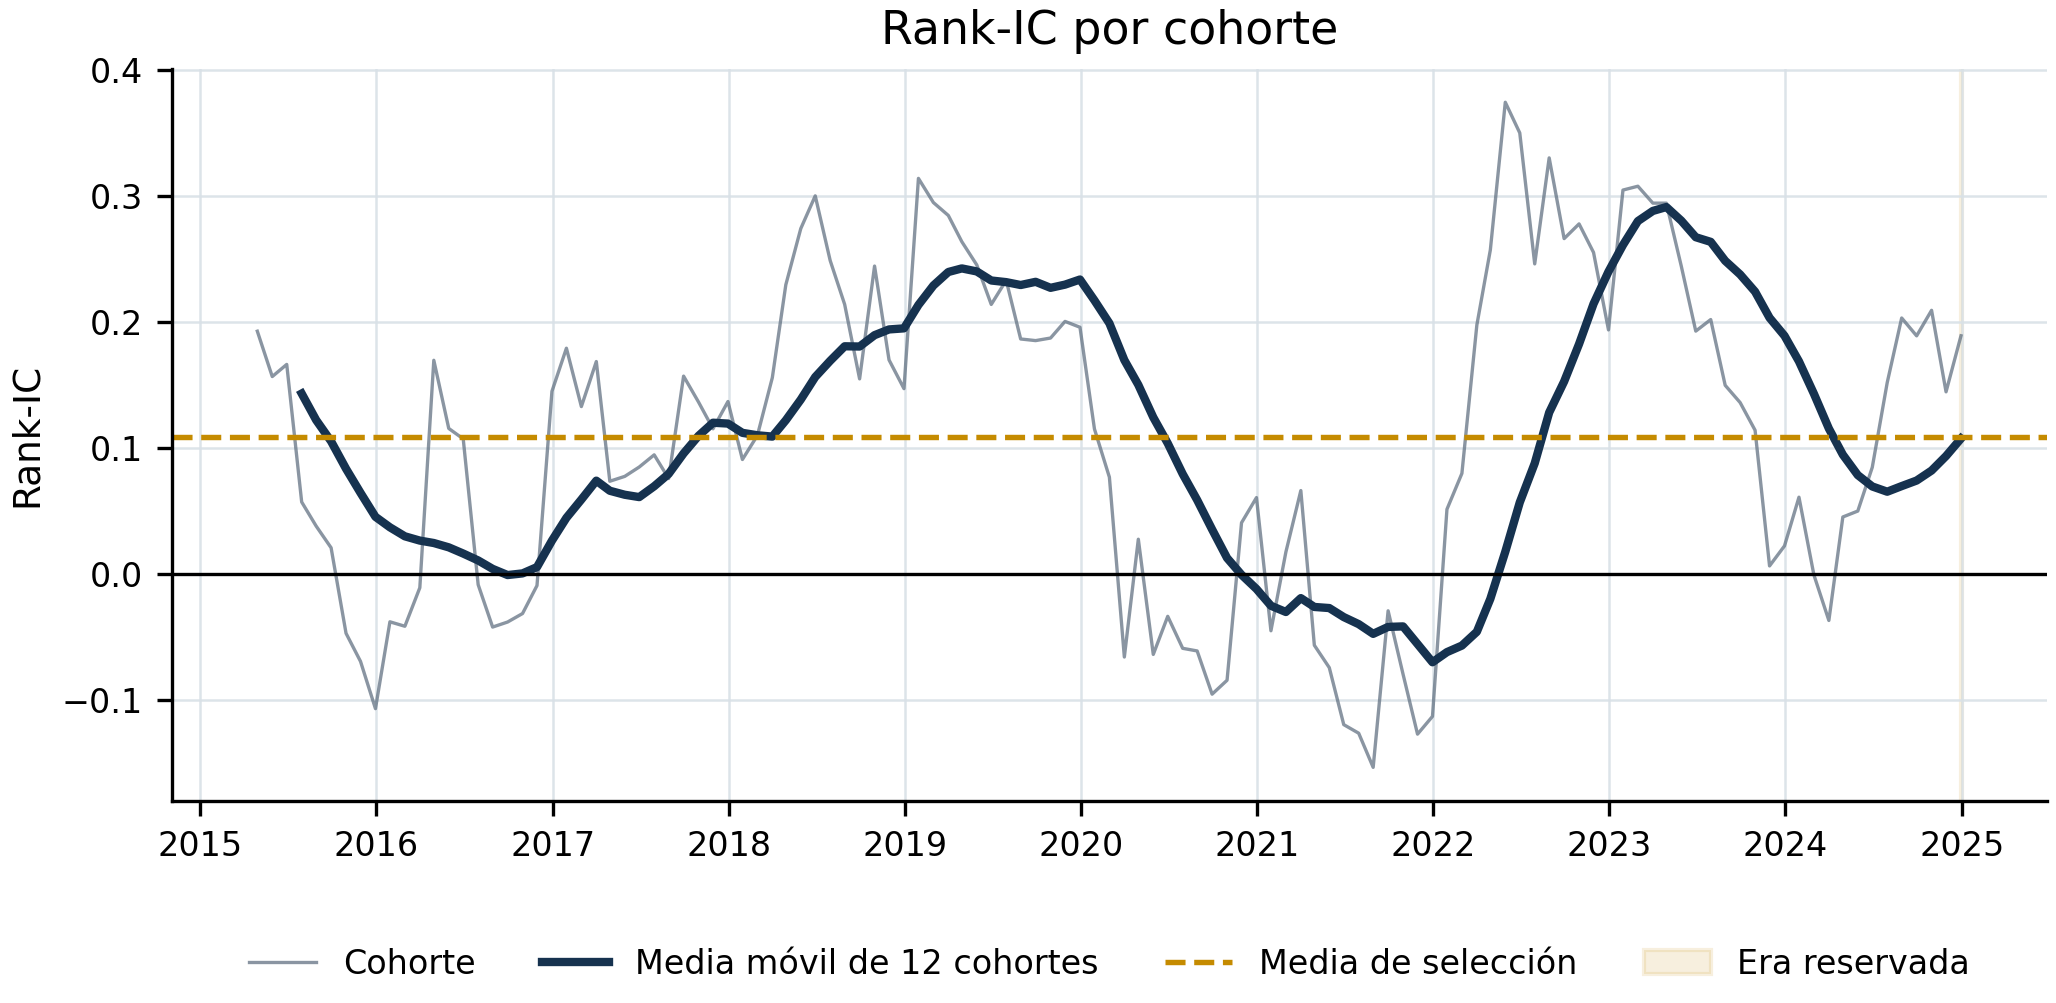
\includegraphics[width=0.96\textwidth]{assets/f07_rankic_serie.png}
  \caption{Rank-IC por cohorte. La banda dorada identifica la era reservada, que no intervino en
  ninguna decisión. Fuente: \texttt{evidence/summary.json}.}
  \label{fig:rankic-serie}
\end{figure}

La comparación limpia se hace contra scores deterministas calculados sobre el mismo panel y con las
mismas restricciones temporales. El mejor, \texttt{garp\_score}, obtiene 0,0130; el sistema lo
multiplica aproximadamente por ocho. No se infiere de ello que los factores clásicos sean inútiles,
sino que, bajo este universo y este protocolo, una combinación no lineal y temporalmente cerrada
ordena mejor los retornos futuros que las fórmulas fijas.

\begin{table}[H]
  \centering
  \caption{Sistema frente a baselines deterministas.}
  \label{tab:baselines}
  \begin{tabular}{lrr}
\toprule
Señal & Rank-IC & Cohortes positivas \\
\midrule
Sistema (meta final) & 0,1067 & 76,07\% \\
garp\_score & 0,0119 & 62,21\% \\
growth\_score & 0,0022 & 51,91\% \\
momentum\_score & -0,0002 & 52,67\% \\
quality\_score & 0,0024 & 52,29\% \\
value\_score & 0,0026 & 48,85\% \\
\bottomrule
\end{tabular}

  \caption*{Fuente: \texttt{attribution.json} y \texttt{evidence/summary.json}.}
\end{table}

Por eras, el Rank-IC es 0,0999 en 2015--2018, 0,0506 en 2019--2021 y 0,1788 en 2022--2024. La
señal se debilita a la mitad en el régimen intermedio, pero no cambia de signo ni depende de la era
final. Esta heterogeneidad justifica reportar series y no una única media agregada, y advierte de
antemano que una media de diez años puede ocultar regímenes en los que el sistema ordena bastante
peor de lo que su cifra agregada sugiere.

\subsection*{La cola superior frente a la ordenación completa}

El Rank-IC resume la calidad de toda la ordenación transversal, pero la cartera sólo compra el
extremo superior. Conviene por tanto comprobar si la ventaja se concentra donde efectivamente se
utiliza. La Tabla~\ref{tab:cola} descompone el comportamiento de la cola por era.

\begin{table}[H]
  \centering
  \small
  \caption{Comportamiento de la cola superior de la ordenación, por era.}
  \label{tab:cola}
  \begin{tabular}{lrrrrrr}
\toprule
Era & Rank-IC & Top 10 & Decil sup. & Universo & Sup. menos inf. & Cohortes \\
\midrule
2015-2018 & 0,0999 & 5,78\% & 4,02\% & -0,26\% & 5,24\% & 45 \\
2019-2021 & 0,0506 & 0,56\% & 1,22\% & -0,00\% & 5,31\% & 36 \\
2022-2024 & 0,1788 & -0,13\% & -1,34\% & -6,47\% & 13,97\% & 36 \\
2025-2026 & 0,0441 & -7,61\% & -7,67\% & -1,85\% & 11,33\% & 6 \\
\bottomrule
\end{tabular}

  \caption*{Fuente: \artefacto{evidence/rank\_tail\_diagnostics.parquet}. «Top 10» es el exceso medio
  de las diez primeras posiciones; «Universo» el de todo el panel. Diagnóstico, no criterio de
  selección.}
\end{table}

La lectura relevante es que el decil superior bate al universo en las tres eras de selección, de
modo que la ventaja no procede exclusivamente de acertar la cola inferior --- que una cartera
\textit{long-only} no puede explotar. La Figura~\ref{fig:cola} muestra esa diferencia cohorte a
cohorte: es ruidosa, como corresponde a un estadístico calculado sobre unas pocas decenas de
valores, pero su media móvil se mantiene por encima de cero durante casi toda la ventana.

\begin{figure}[H]
  \centering
  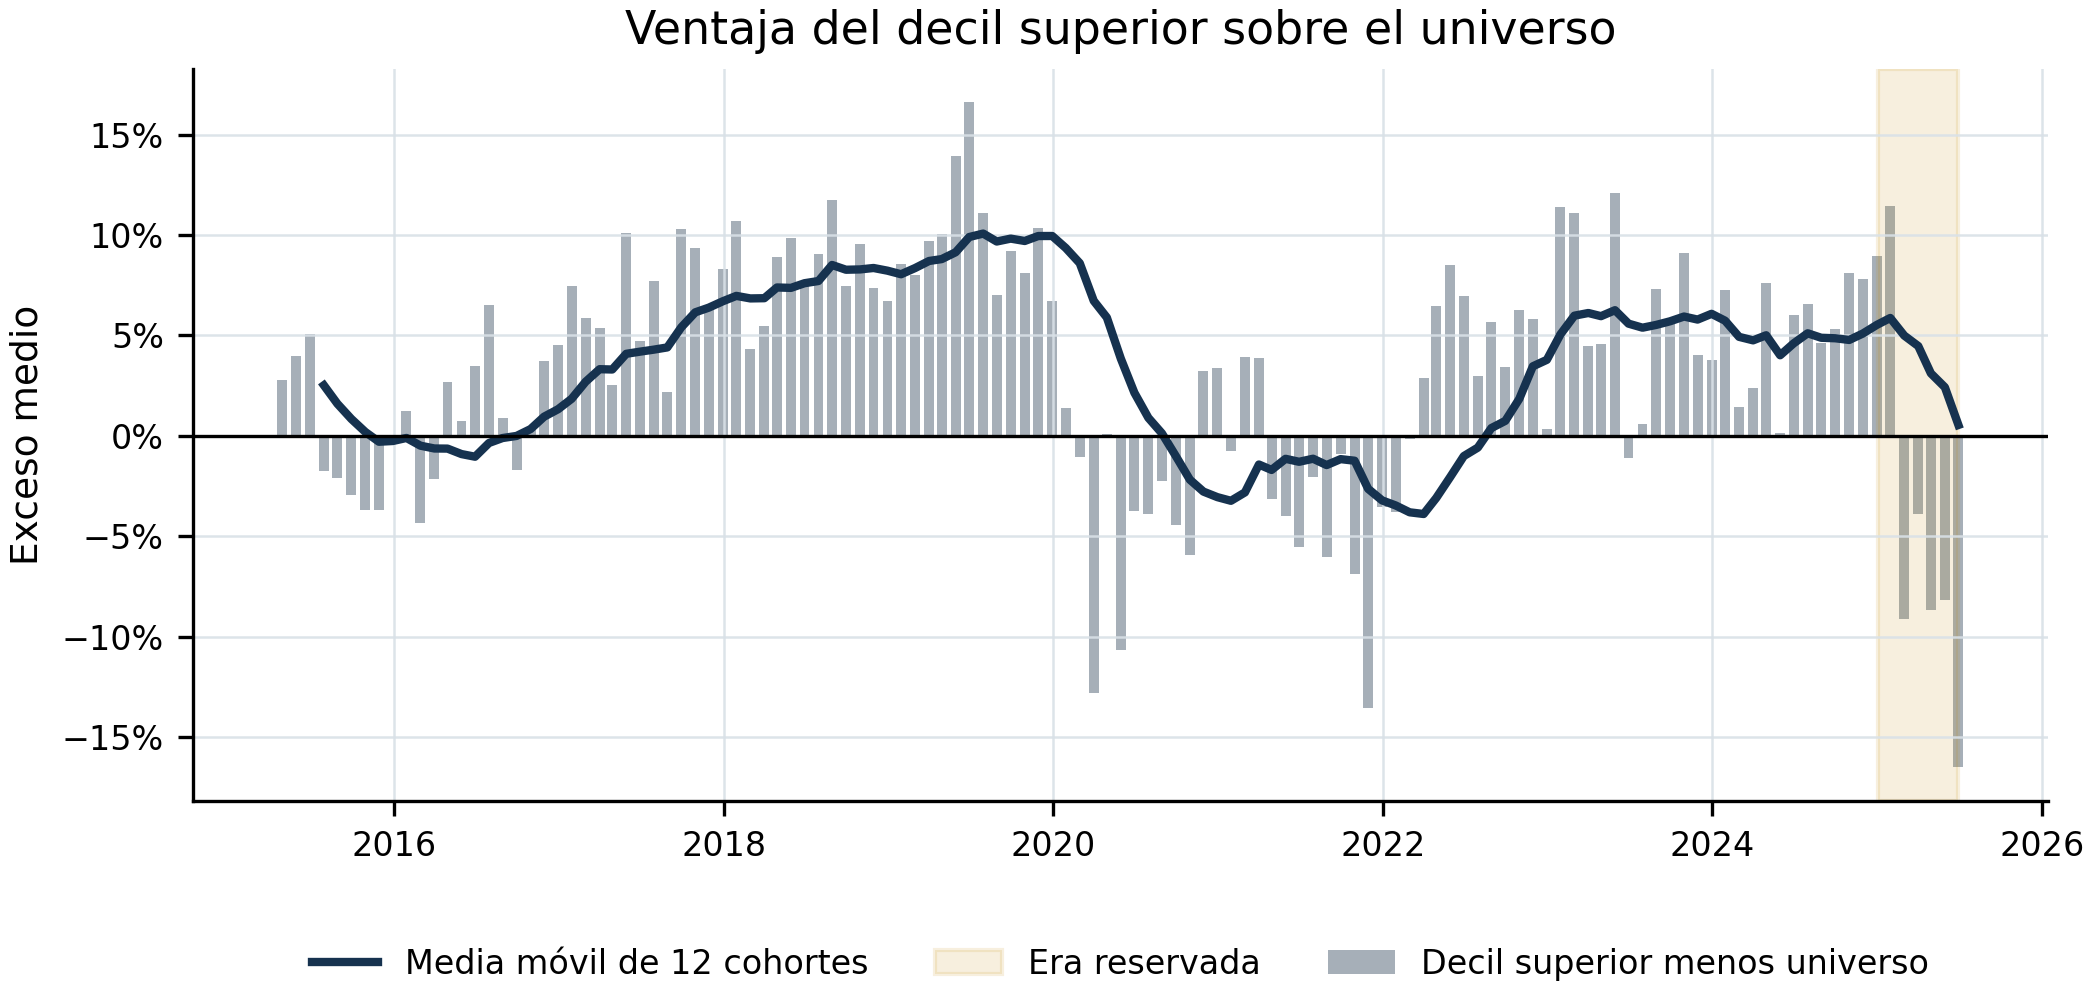
\includegraphics[width=0.94\textwidth]{assets/f07_cola.png}
  \caption{Exceso del decil superior sobre el universo, por cohorte. Fuente:
  \artefacto{evidence/rank\_tail\_diagnostics.parquet}.}
  \label{fig:cola}
\end{figure}

Existe además un diagnóstico que el sistema calcula en cada snapshot para su propio uso: el Rank-IC
contraído sobre las cohortes ya cerradas en ese momento. Es la única medida de calidad de señal
disponible \textit{en tiempo real}, puesto que no utiliza información posterior a la fecha. La
Figura~\ref{fig:salud} la representa con dos memorias distintas.

\begin{figure}[H]
  \centering
  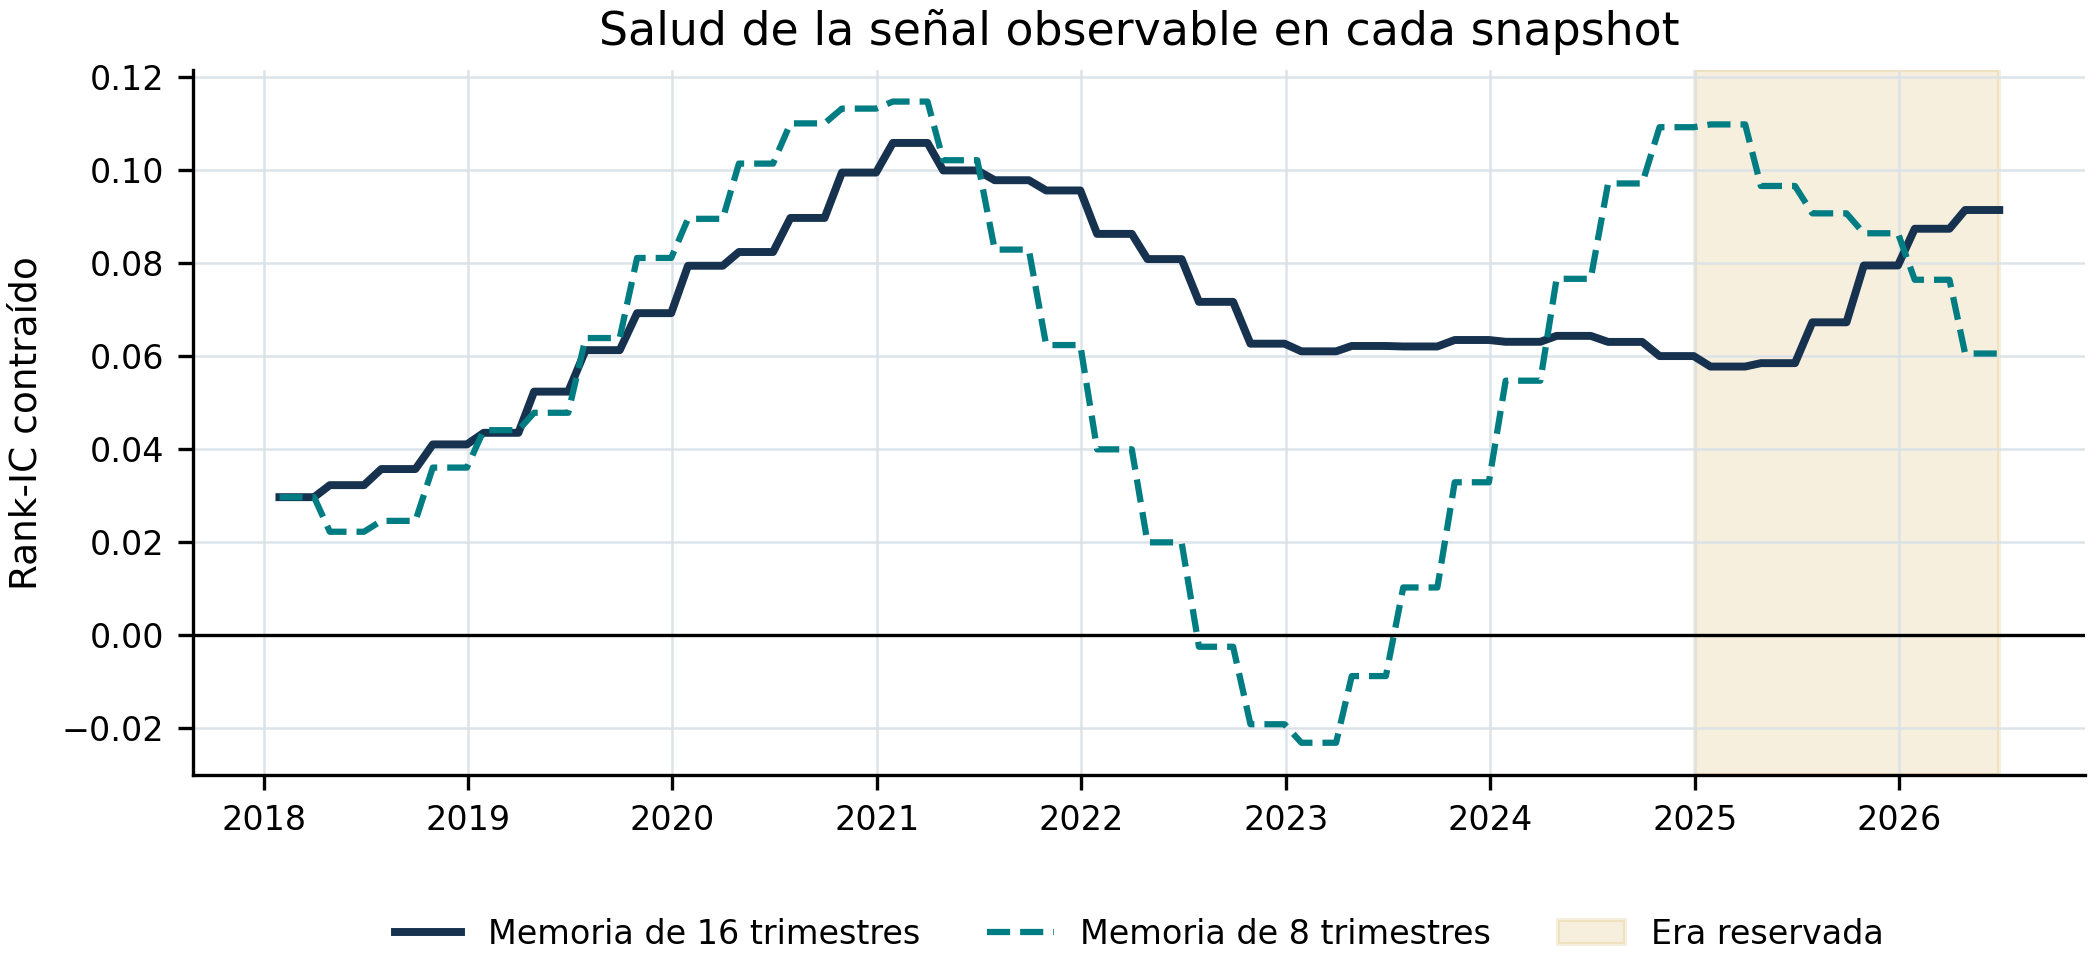
\includegraphics[width=0.94\textwidth]{assets/f07_salud.png}
  \caption{Salud de la señal observable en cada snapshot, con memoria de dieciséis y de ocho
  trimestres. Fuente: \artefacto{evidence/signal\_health.parquet}.}
  \label{fig:salud}
\end{figure}

La comparación entre ambas memorias es informativa por sí misma. La ventana corta reacciona antes a
los cambios de régimen, pero también oscila más y llega a cruzar cero en episodios que la ventana
larga apenas registra. Esta diferencia explica por qué el catálogo trata la longitud de la memoria
del meta-agente como una variable a decidir con evidencia y no como una constante razonable: ambas
opciones tienen un coste, y la elección entre reaccionar antes o estimar con menos varianza no
puede resolverse por intuición.

\section{Robustez: aprendizaje y no suerte}

La Tabla~\ref{tab:robustez} resume ocho contrastes predefinidos. Siete respaldan la capacidad
predictiva; el Deflated Sharpe no alcanza su umbral de 0,95. Reportar este último resultado evita
convertir la robustez en una lista selectiva de éxitos: la evidencia de señal y la evidencia de
rentabilidad ajustada por multiplicidad no tienen la misma fuerza.

\begin{table}[H]
  \centering
  \caption{Resumen de contrastes de robustez.}
  \label{tab:robustez}
  \begin{tabular}{llc}
\toprule
Contraste & Resultado & Veredicto \\
\midrule
Permutación & $p=0,0001$; 9.999 réplicas & Supera \\
Placebos & Rank-IC entre $-0,0081$ y $0,0013$ & Supera \\
Bootstrap & IC 95\% $[0,0425; 0,1723]$ & Supera \\
Exclusión de eras & Rank-IC entre $0,0780$ y $0,1350$ & Supera \\
Semillas & Rango de Rank-IC $0,0015$ & Supera \\
Aleatorias con riesgo & Percentil $96,8$ & Supera \\
Neutralización & Retiene 86,62\% de la señal & Supera \\
Deflated Sharpe & $0,682 < 0,95$ & No supera \\
\bottomrule
\end{tabular}

  \caption*{Fuente: \texttt{robustness.json} y \texttt{attribution.json}. Los contrastes de señal no
  dependen de la cartera; el Deflated Sharpe y las carteras aleatorias, que sí, están calculados
  sobre la cartera del Model Study.}
\end{table}

\begin{figure}[H]
  \centering
  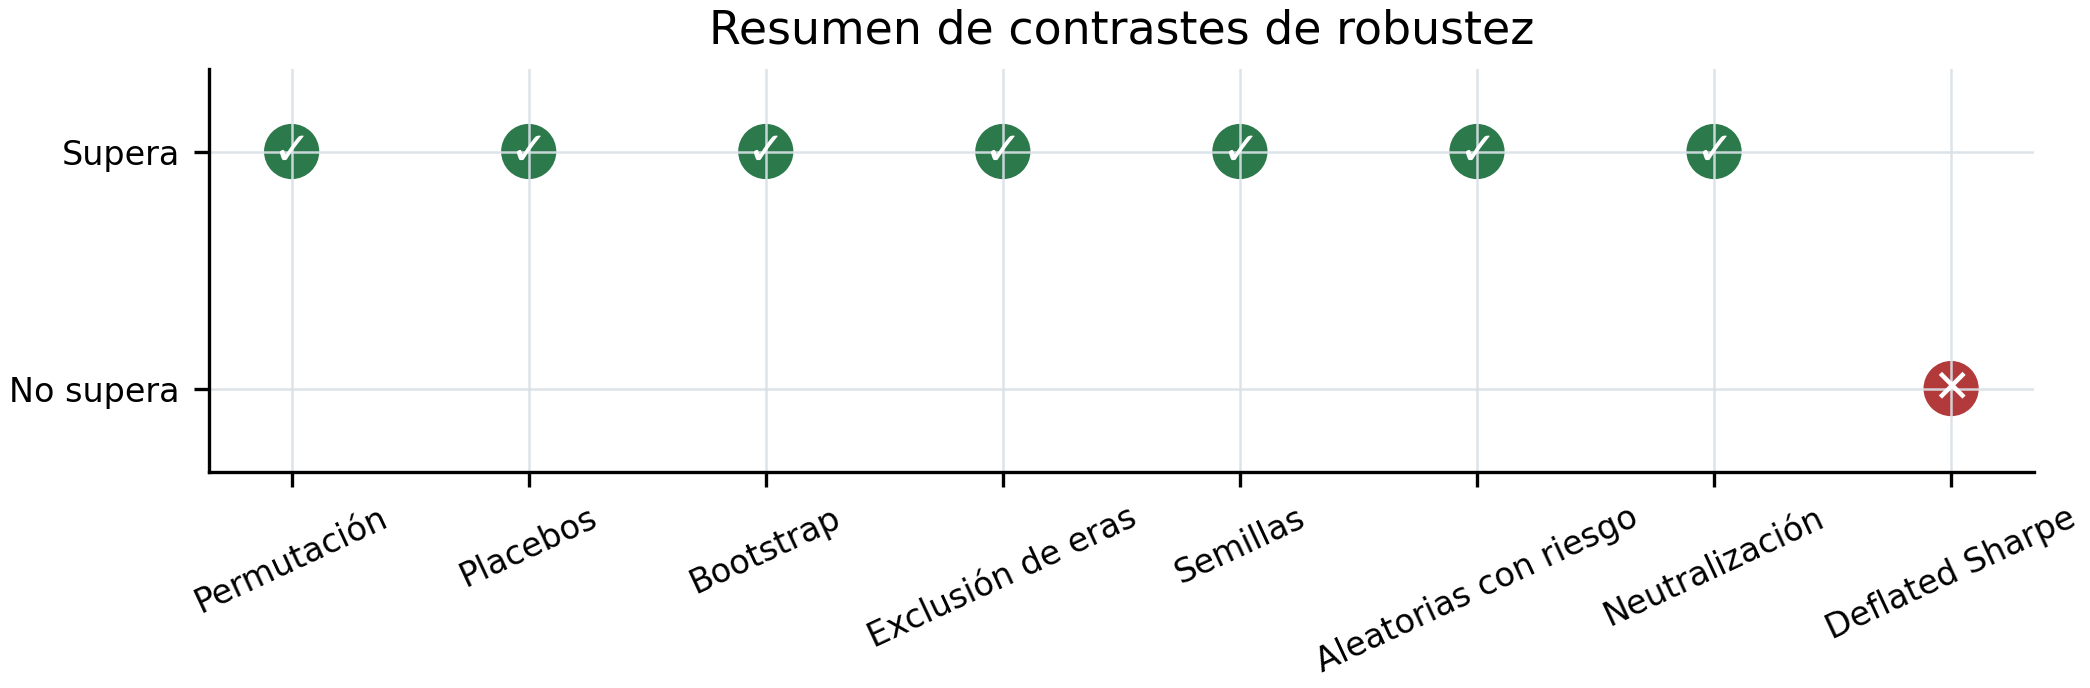
\includegraphics[width=0.92\textwidth]{assets/f07_robustez.png}
  \caption{Veredicto de los ocho contrastes. La figura sintetiza los estadísticos persistidos; los
  valores exactos y su interpretación se detallan en la Tabla~\ref{tab:robustez}.}
  \label{fig:robustez}
\end{figure}

El test de permutación entrega $p=0,0001$ con 9.999 réplicas y corrección +1: ninguna réplica
igualó el Rank-IC observado. La permutación destruye únicamente el vínculo entre el orden predicho
y el retorno futuro dentro de cada cohorte, conservando el calendario, el número de empresas y la
distribución transversal de los retornos. Responde por tanto a una pregunta muy concreta: ¿puede
surgir un Rank-IC como el observado sin ninguna asociación predictiva? Con 9.999 réplicas y ninguna
que lo alcance, la respuesta empírica es que no.

Los cinco placebos de etiqueta son complementarios y atacan otra objeción. Conservan la maquinaria
completa de features, agentes, meta-agente y cartera, pero sustituyen la etiqueta por una barajada.
Si alguna parte del \textit{pipeline} fabricase señal por sí misma --- una normalización mal
cerrada, una fuga temporal, un artefacto de la validación ---, los placebos deberían mostrar una
magnitud comparable a la observada. Quedan entre $-0,0061$ y $+0,0008$, es decir, indistinguibles de
cero y dos órdenes de magnitud por debajo del sistema.

\begin{figure}[H]
  \centering
  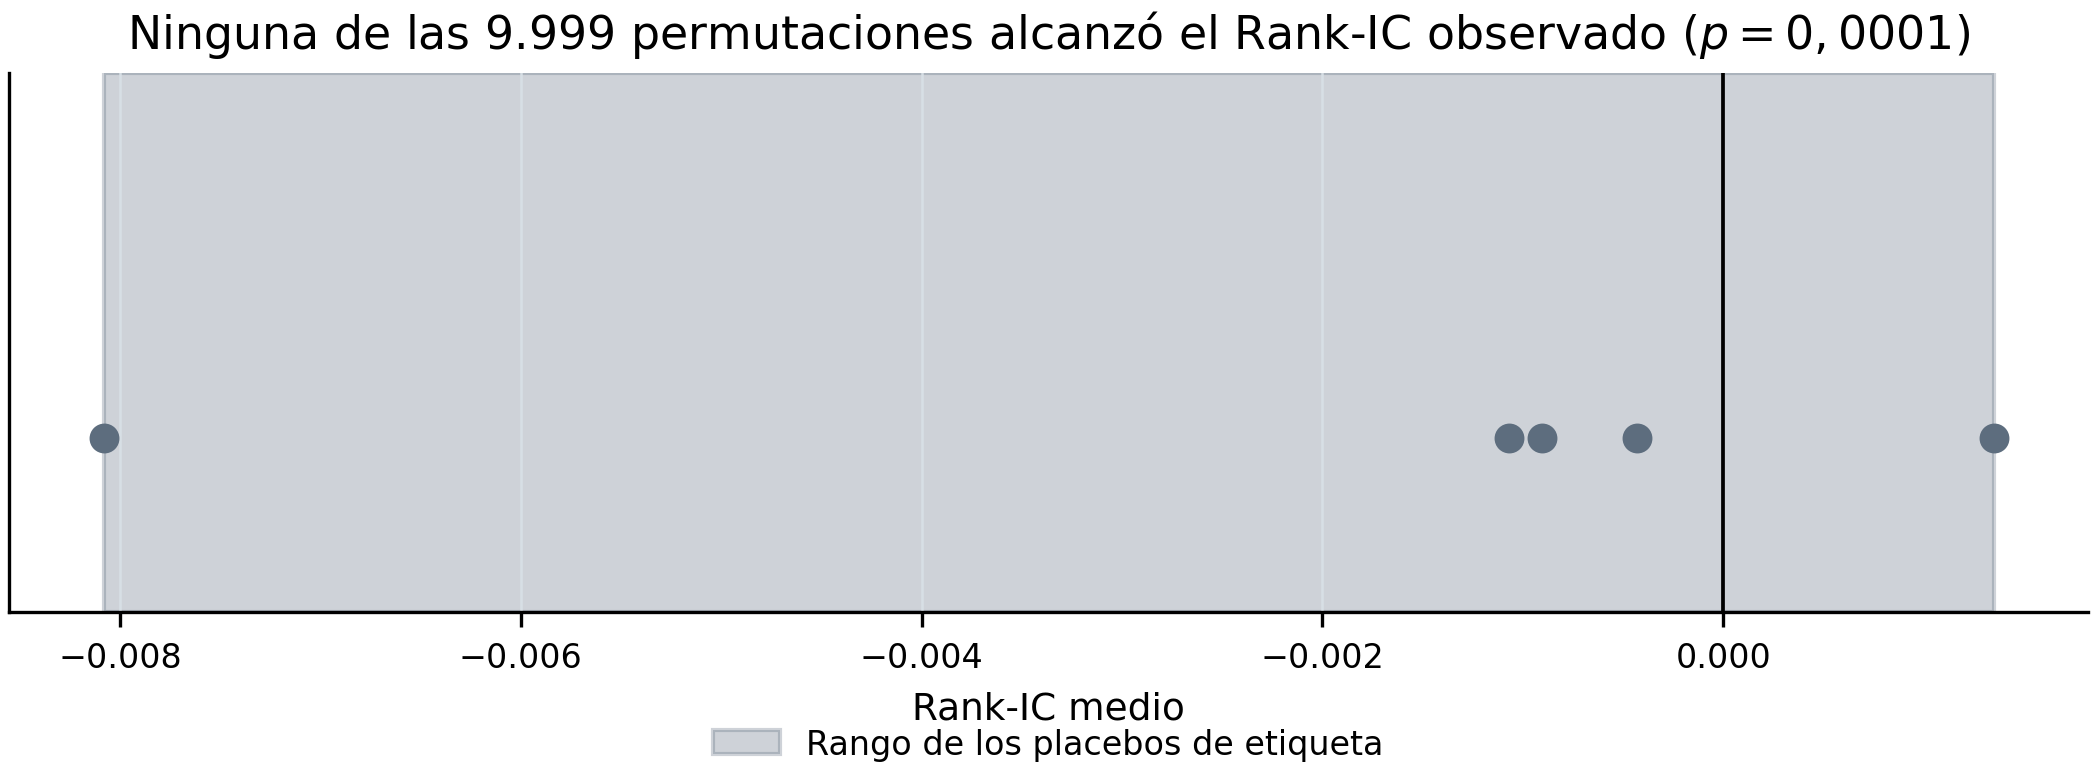
\includegraphics[width=0.94\textwidth]{assets/f07_permutacion.png}
  \caption{Situación del Rank-IC observado frente al rango de los placebos de etiqueta y al
  resultado del contraste de permutación. Fuente: \artefacto{robustness.json}.}
  \label{fig:permutacion}
\end{figure}

\begin{figure}[H]
  \centering
  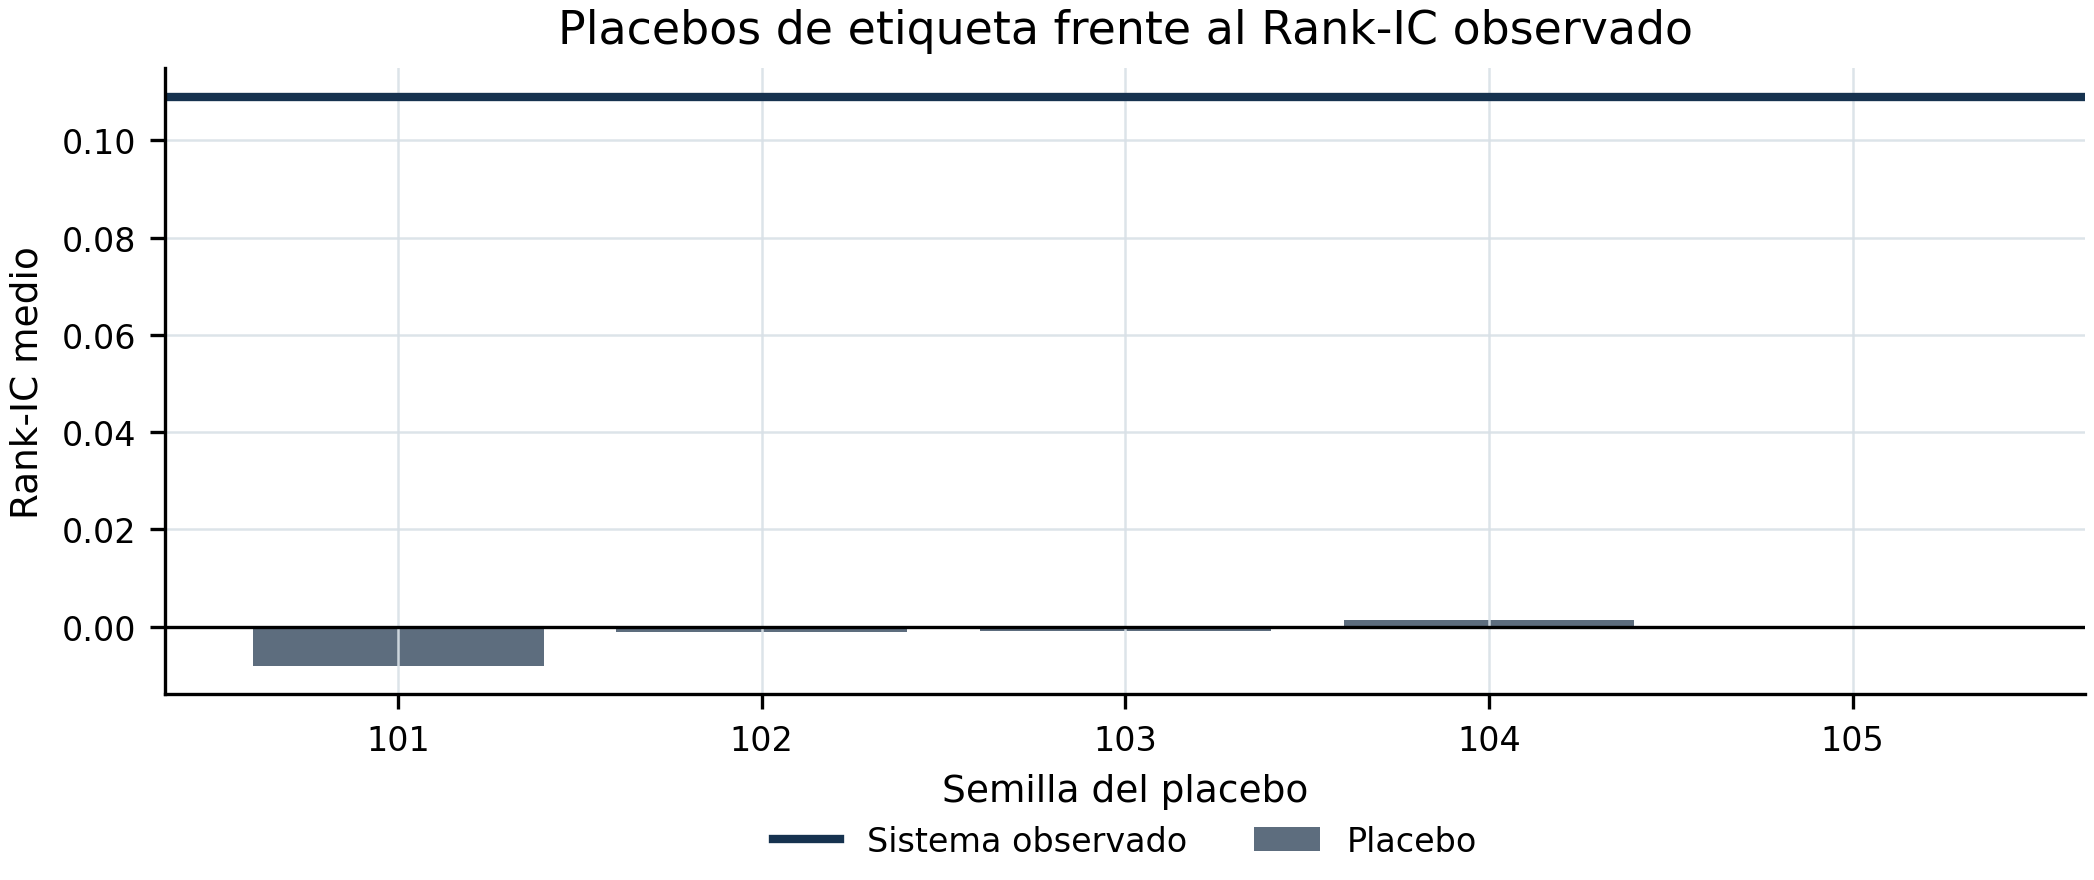
\includegraphics[width=0.88\textwidth]{assets/f07_placebos.png}
  \caption{Placebos de etiqueta y Rank-IC del sistema. Fuente: \artefacto{robustness.json}.}
  \label{fig:placebos}
\end{figure}

La Figura~\ref{fig:permutacion} representa la distribución nula completa: el estudio persiste los
estadísticos de las 9.999 permutaciones, no sólo el $p$-valor resultante, de modo que puede verse
dónde cae el Rank-IC observado dentro de la nube de permutaciones y no únicamente que la supera. El
$p$-valor del texto se recalcula exactamente desde esas réplicas. El Anexo~\ref{anexo:evidencia}
detalla qué se guarda de cada contraste.

El \textit{bootstrap} por bloques y la exclusión de eras responden a una tercera objeción: que una
media positiva esté dominada por meses correlacionados o por un subperiodo excepcional. Manteniendo
bloques de doce cohortes --- la longitud del horizonte, precisamente para no romper la dependencia
que el solapamiento induce ---, el intervalo al 95\,\% es $[0,0335;\,0,1695]$ y excluye cero.
Eliminando por completo cualquiera de las tres eras, la media permanece entre 0,0730 y 0,1262. La
Figura~\ref{fig:bootstrap} reúne ambos contrastes.

\begin{figure}[H]
  \centering
  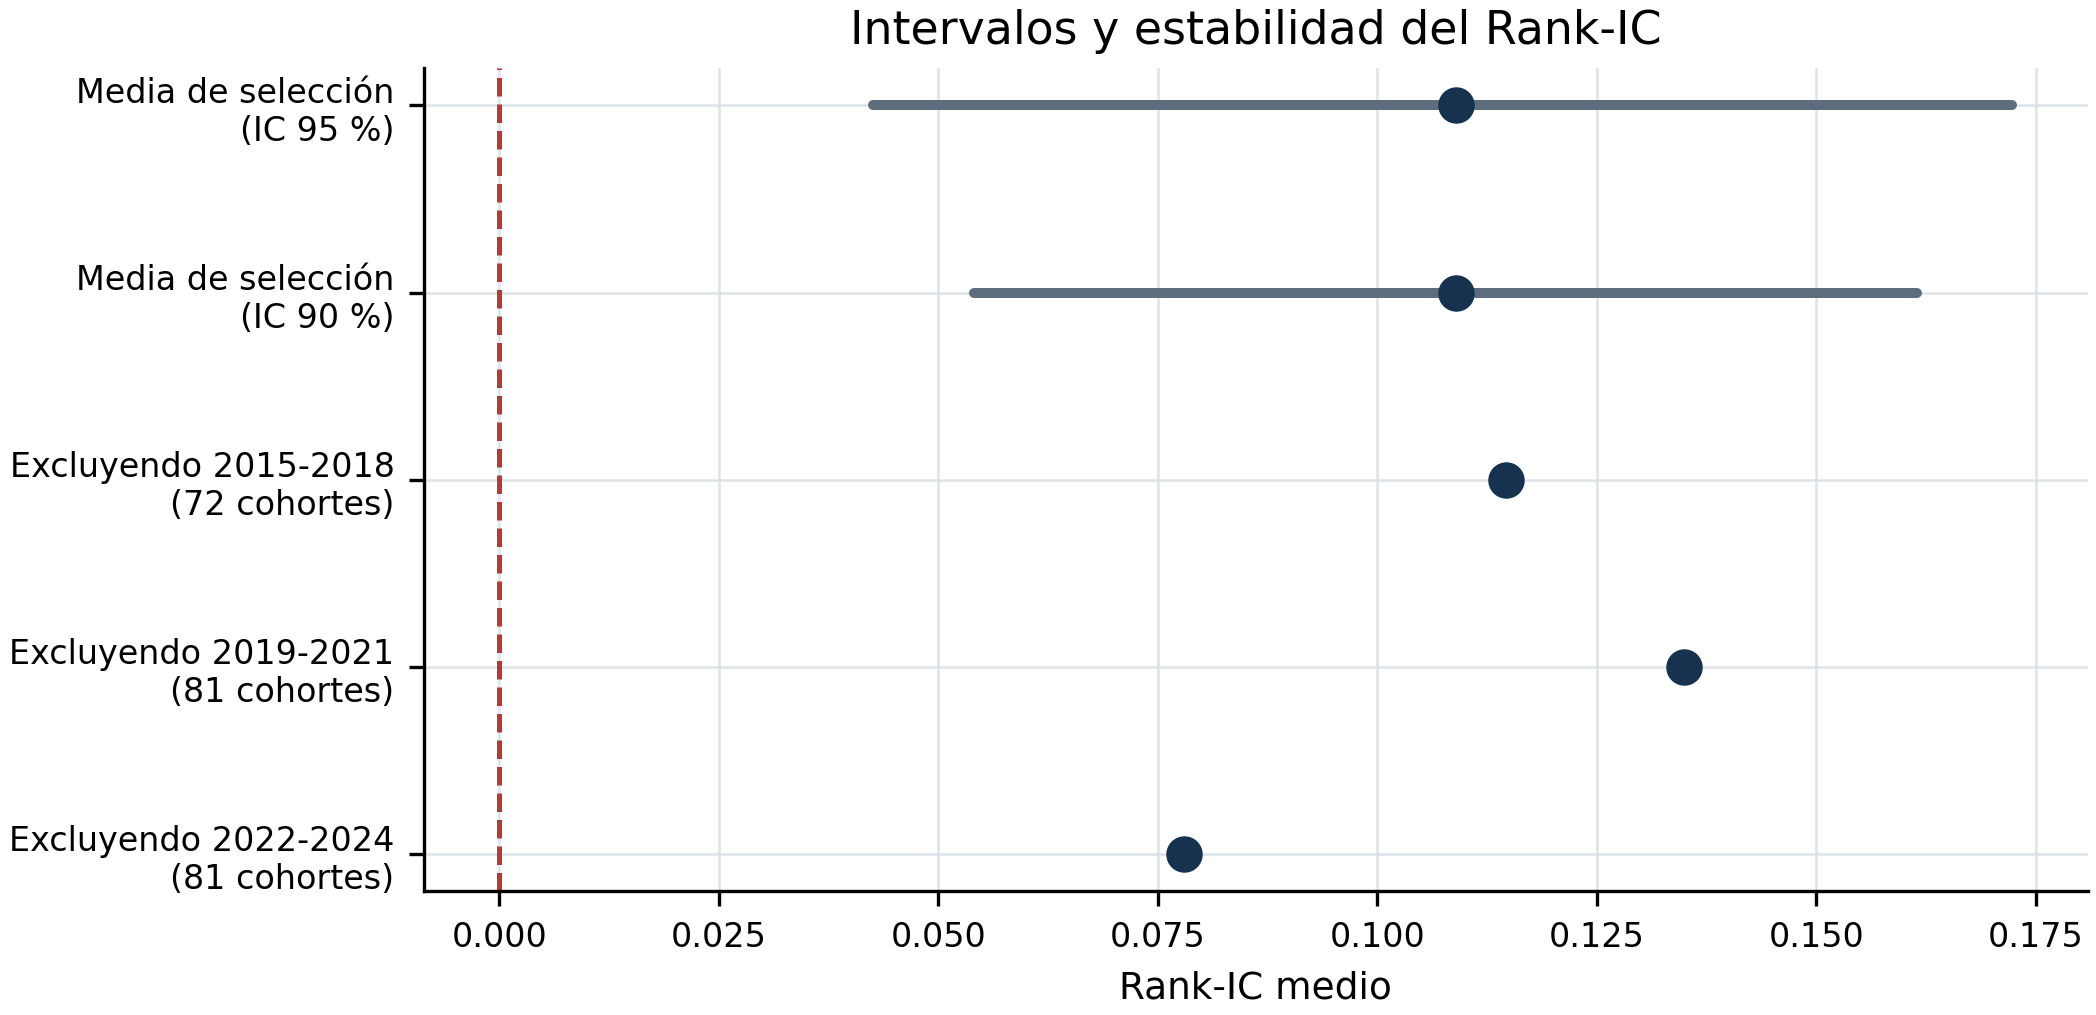
\includegraphics[width=0.94\textwidth]{assets/f07_bootstrap.png}
  \caption{Intervalos de confianza del Rank-IC y estabilidad ante la exclusión de eras completas.
  Fuente: \artefacto{robustness.json}.}
  \label{fig:bootstrap}
\end{figure}

\begin{table}[H]
  \centering
  \small
  \caption{Intervalos, exclusión de eras y dispersión entre semillas.}
  \label{tab:eras-bootstrap}
  \begin{tabular}{lrccr}
\toprule
Contraste & Valor central & Intervalo 90\% & Intervalo 95\% & Obs. \\
\midrule
Media de selección & 0,1004 & [0,0449; 0,1585] & [0,0335; 0,1695] & 117 \\
Excluyendo 2015-2018 & 0,1022 & — & — & 72 \\
Excluyendo 2019-2021 & 0,1262 & — & — & 81 \\
Excluyendo 2022-2024 & 0,0730 & — & — & 81 \\
Rank-IC entre semillas & 0,0989 & [0,0984; 0,1004] & — & 3 \\
IR entre semillas & 0,269 & [0,182; 0,269] & — & 3 \\
\bottomrule
\end{tabular}

  \caption*{Fuente: \artefacto{robustness.json}. La exclusión de eras reajusta el sistema sobre el
  resto de la ventana; las semillas reejecutan el estudio completo.}
\end{table}

El contraste más exigente de la era 2022--2024 merece una nota: al excluirla, el Rank-IC cae a
0,0730, el valor más bajo de los tres. Es coherente con que sea la era de mayor señal (0,1621) y no
indica fragilidad, sino que esa era aporta una parte apreciable de la evidencia. La conclusión
prudente es que el resultado no depende de ninguna era, pero tampoco es homogéneo entre ellas.

La estabilidad entre semillas ataca una posibilidad distinta: que el resultado dependa de una
inicialización afortunada del \textit{boosting}. En las tres semillas ensayadas el rango de Rank-IC
es 0,0020 y no cruza cero. La Figura~\ref{fig:semillas} muestra, sin embargo, que la conclusión
económica es bastante más frágil que la predictiva: el exceso geométrico varía apreciablemente más
que el Rank-IC en términos relativos. Esta asimetría es la misma que motivó introducir el conjunto
de semillas durante el desarrollo, según se documenta en el Capítulo~\ref{chap:desarrollo-metodo}.

\begin{figure}[H]
  \centering
  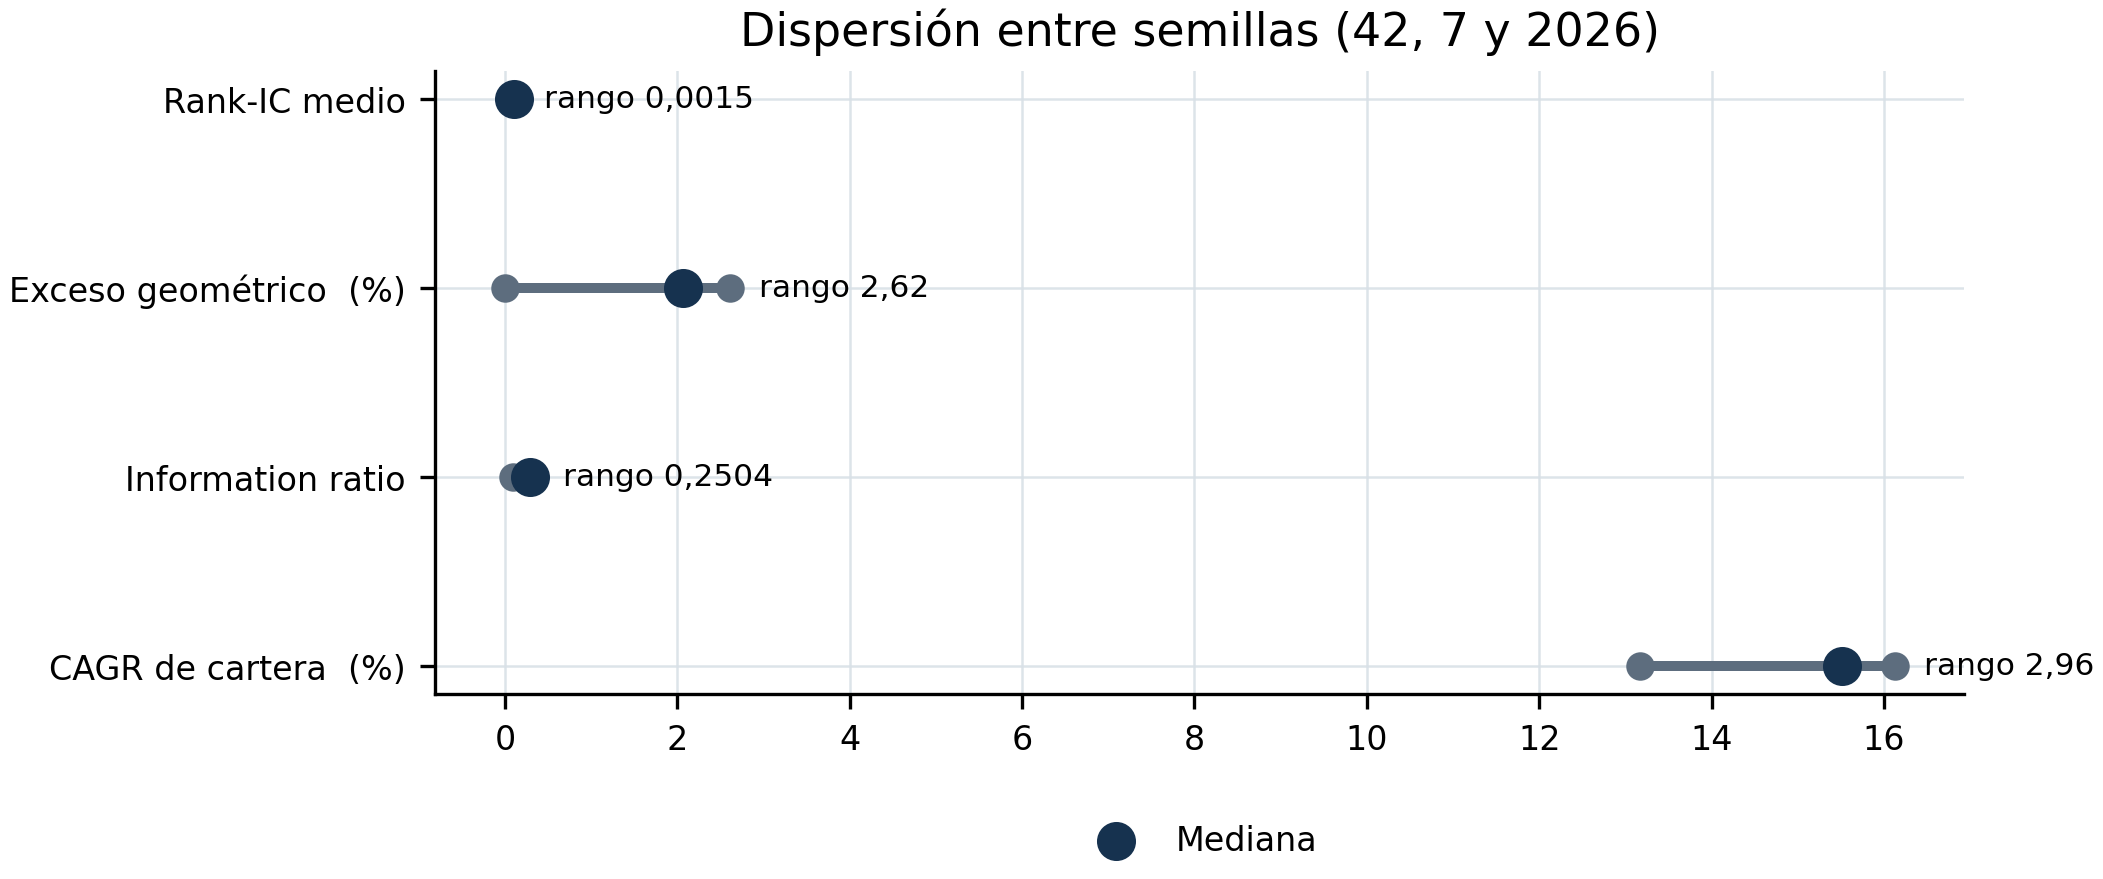
\includegraphics[width=0.92\textwidth]{assets/f07_semillas.png}
  \caption{Dispersión de las métricas principales entre las tres semillas ensayadas. Fuente:
  \artefacto{robustness.json}.}
  \label{fig:semillas}
\end{figure}

Frente a 1.000 carteras aleatorias de riesgo emparejado, la cartera del modelo ocupa el percentil
97,4. El contraste aleatorio general no se usa como prueba favorable, y conviene explicar por qué:
su percentil 95 de CAGR es 102,28\,\%, dominado por carteras que por azar concentraron alguna
superviviente extraordinaria. Un nulo con esa cola no es un \textit{benchmark} informativo, y
presentarlo como si el modelo «sólo» alcanzase el percentil 65 sería tan engañoso como omitirlo. La
Figura~\ref{fig:aleatorias} muestra los dos escenarios juntos precisamente para que la diferencia
sea visible.

\begin{figure}[H]
  \centering
  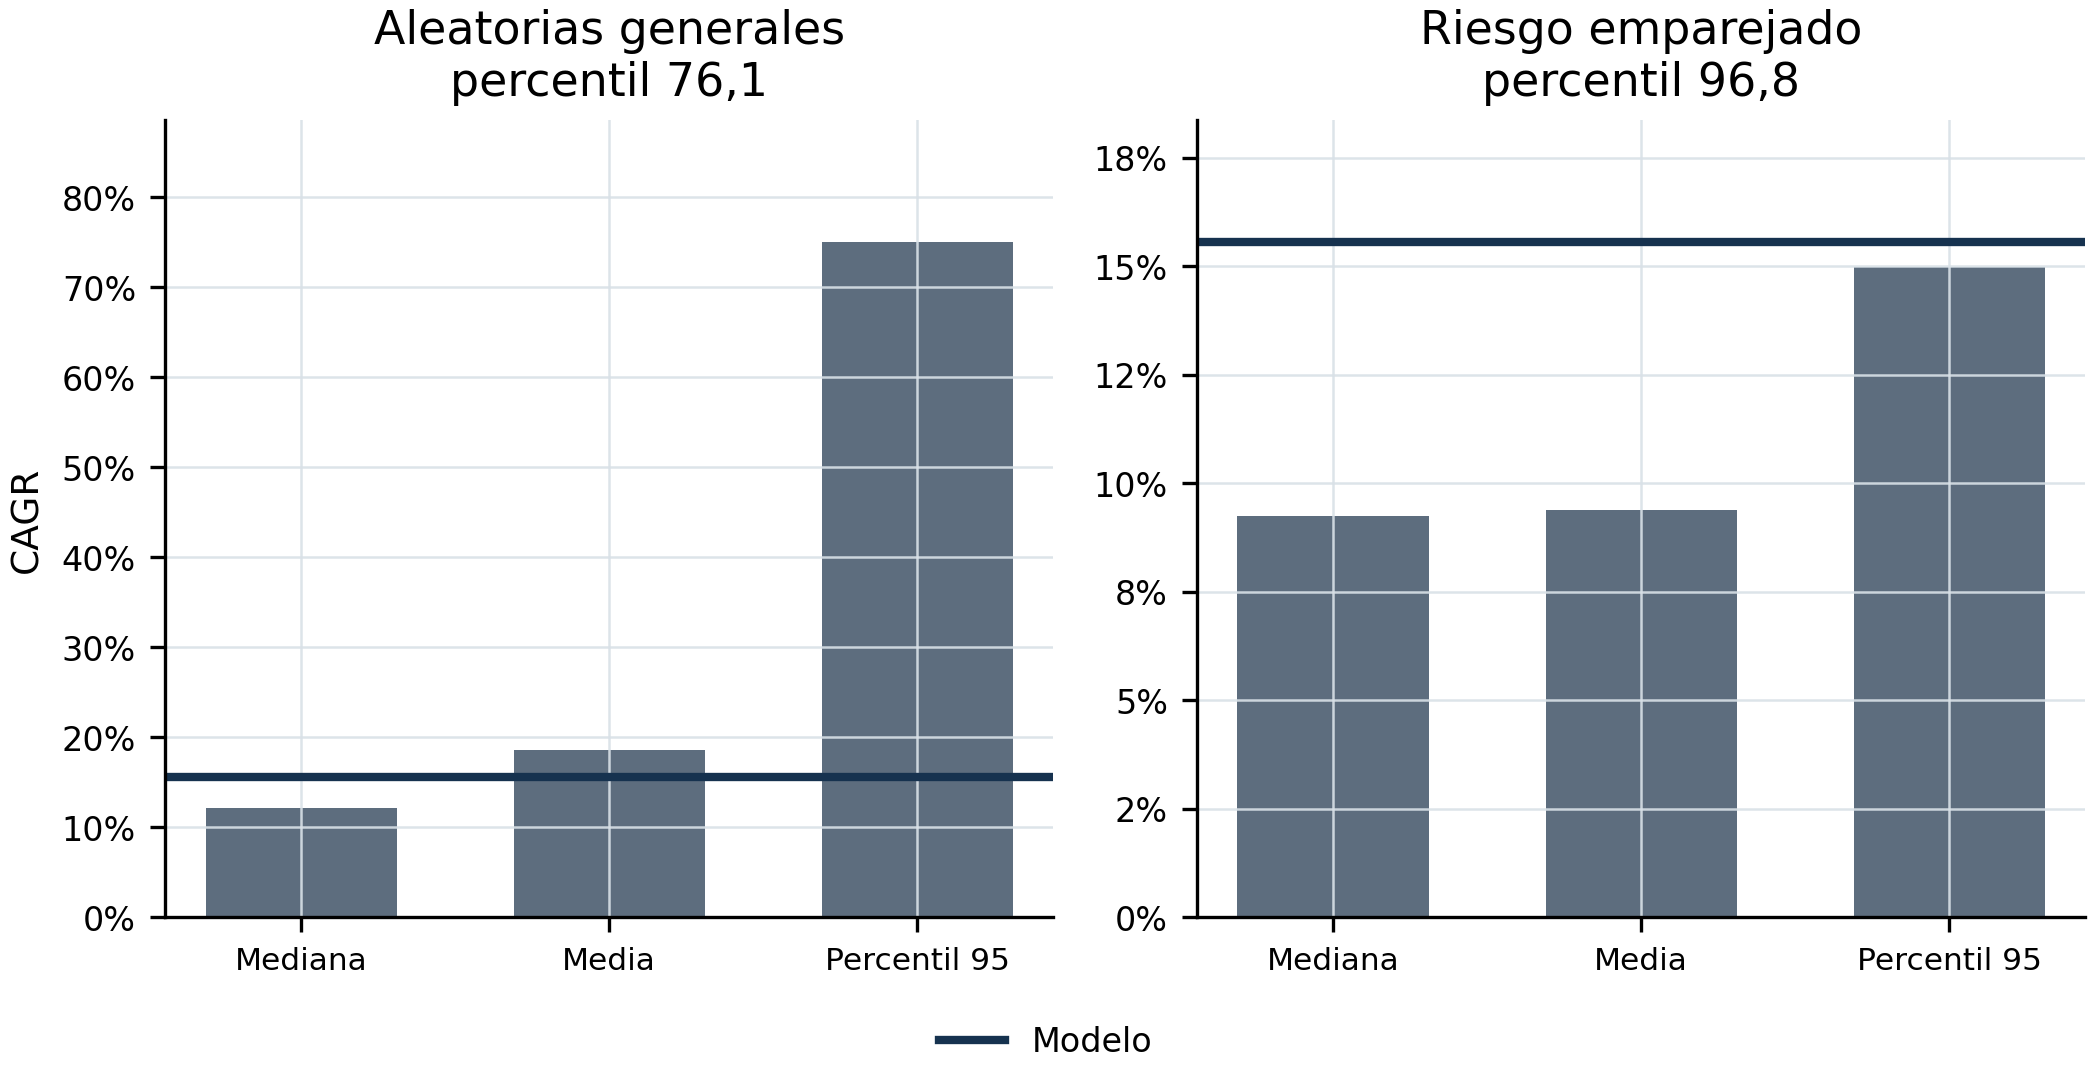
\includegraphics[width=0.92\textwidth]{assets/f07_aleatorias.png}
  \caption{Cartera del modelo frente a 1.000 carteras aleatorias, en el escenario general y con
  riesgo emparejado. Fuente: \artefacto{robustness.json}.}
  \label{fig:aleatorias}
\end{figure}

La neutralización por controles de estilo reduce el Rank-IC de 0,1177 a 0,1019; por tanto se
retiene 86,62\% de la señal. La regresión factorial de la ventana de selección produce alfa por
periodo 0,27\%, $t=1,44$ y $R^2=0,017$. No hay evidencia suficiente para atribuir ese alfa a un
factor clásico, pero tampoco para afirmar que sea significativo por sí mismo.

\section{Traducción económica y confirmación reservada}

Una vez congelada la señal y optimizada la cartera --- el procedimiento se describe en la
Sección~\ref{sec:cartera-rejilla} y sus resultados se analizan allí ---, la cartera obtiene entre
2015 y 2024 CAGR 21,06\% frente a 13,17\% de SPY; el exceso geométrico es 6,97\%, el IR 0,844, el
máximo drawdown 28,40\% y el benchmark se bate en 8 de 10 años. El coste acumulado, 4,74\%, y el
turnover anualizado, 324,43\%, son centrales para interpretar el resultado: la implementación
captura sólo una parte de la señal disponible, y lo hace pagando fricción por el camino.

Conviene declarar de entrada, para que ninguna de estas cifras se lea como más limpia de lo que es,
que la configuración de cartera que las produce fue elegida por su Information Ratio sobre esta
misma ventana 2015--2024. Están, por tanto, contaminadas por esa selección igual que las cifras
predictivas lo están por la suya. La comprobación que no lo está es la de la era reservada, y se
presenta más adelante en este capítulo.

Antes de entrar en el detalle conviene fijar una convención de lectura que el resto del capítulo
respeta. Toda cifra económica de este trabajo pertenece a una de tres ventanas con estatus
epistemológico distinto, y mezclarlas produce afirmaciones que no se sostienen. La ventana de
\emph{selección} (2015--2024) es donde se tomaron las diecisiete decisiones: sus cifras describen
el sistema, pero están contaminadas por esa selección. La ventana de \emph{confirmación}
(2025--2026) no intervino en ninguna decisión, de modo que sus cifras son honestamente fuera de
muestra, pero son pocas. La \emph{curva completa} sirve para describir la serie histórica en su
conjunto y no debe usarse como evidencia de nada, porque mezcla ambos regímenes. La
Tabla~\ref{tab:tres-ventanas} las presenta separadas y etiquetadas.

\begin{table}[H]
  \centering
  \small
  \caption{Las tres ventanas de evaluación, con su papel declarado.}
  \label{tab:tres-ventanas}
  \begin{tabular}{lrrr}
\toprule
Métrica & Selección 2015–2024 & Confirmación 2025–2026 & Curva completa \\
\midrule
CAGR de cartera & 21,06\% & 22,23\% & 21,04\% \\
CAGR de SPY & 13,17\% & 19,18\% & 13,81\% \\
Exceso geométrico & 6,97\% & 2,56\% & 6,35\% \\
Information ratio & 0,844 & 0,304 & 0,753 \\
Máximo drawdown & 28,40\% & 12,09\% & 28,40\% \\
Años por encima de SPY & 80,00\% & 50,00\% & 75,00\% \\
Alfa anual media & 7,17\% & 1,91\% & 6,29\% \\
Peor alfa anual & -8,30\% & -2,73\% & -8,30\% \\
Turnover anualizado & 324,43\% & 391,35\% & 333,35\% \\
Efectivo medio & 0,00\% & 0,00\% & 0,00\% \\
Coste acumulado & 4,74\% & 0,88\% & 5,63\% \\
Periodos & 117 & 18 & 135 \\
\bottomrule
\end{tabular}

  \caption*{Fuente: \artefacto{evidence\_best\_full/summary.json} del ganador del Portfolio Study:
  son cifras de la cartera adoptada, no de la que el catálogo recomienda. Selección: se tomaron
  decisiones sobre ella. Confirmación: reservada, ninguna decisión la utilizó. Curva completa:
  descriptiva, no probatoria.}
\end{table}

Dos observaciones sobre la tabla condicionan su lectura. La primera es que el efectivo medio es
\textbf{cero en las tres ventanas}: la cartera ganadora renuncia por completo a la liquidez, de modo
que su resultado no puede atribuirse a haber estado fuera del mercado en los momentos oportunos.
Está siempre invertida, y su exceso procede íntegramente de qué acciones eligió.

La segunda es que el turnover \emph{sube} en la era reservada, de 324\,\% a 391\,\%, mientras el
coste acumulado se mantiene bajo por lo corto del periodo. No hay aquí un cambio de comportamiento
del sistema: con una cartera de ocho posiciones y sin colchón de efectivo, cada cambio de opinión de
la señal obliga a una rotación completa de la plaza afectada.

\begin{figure}[H]
  \centering
  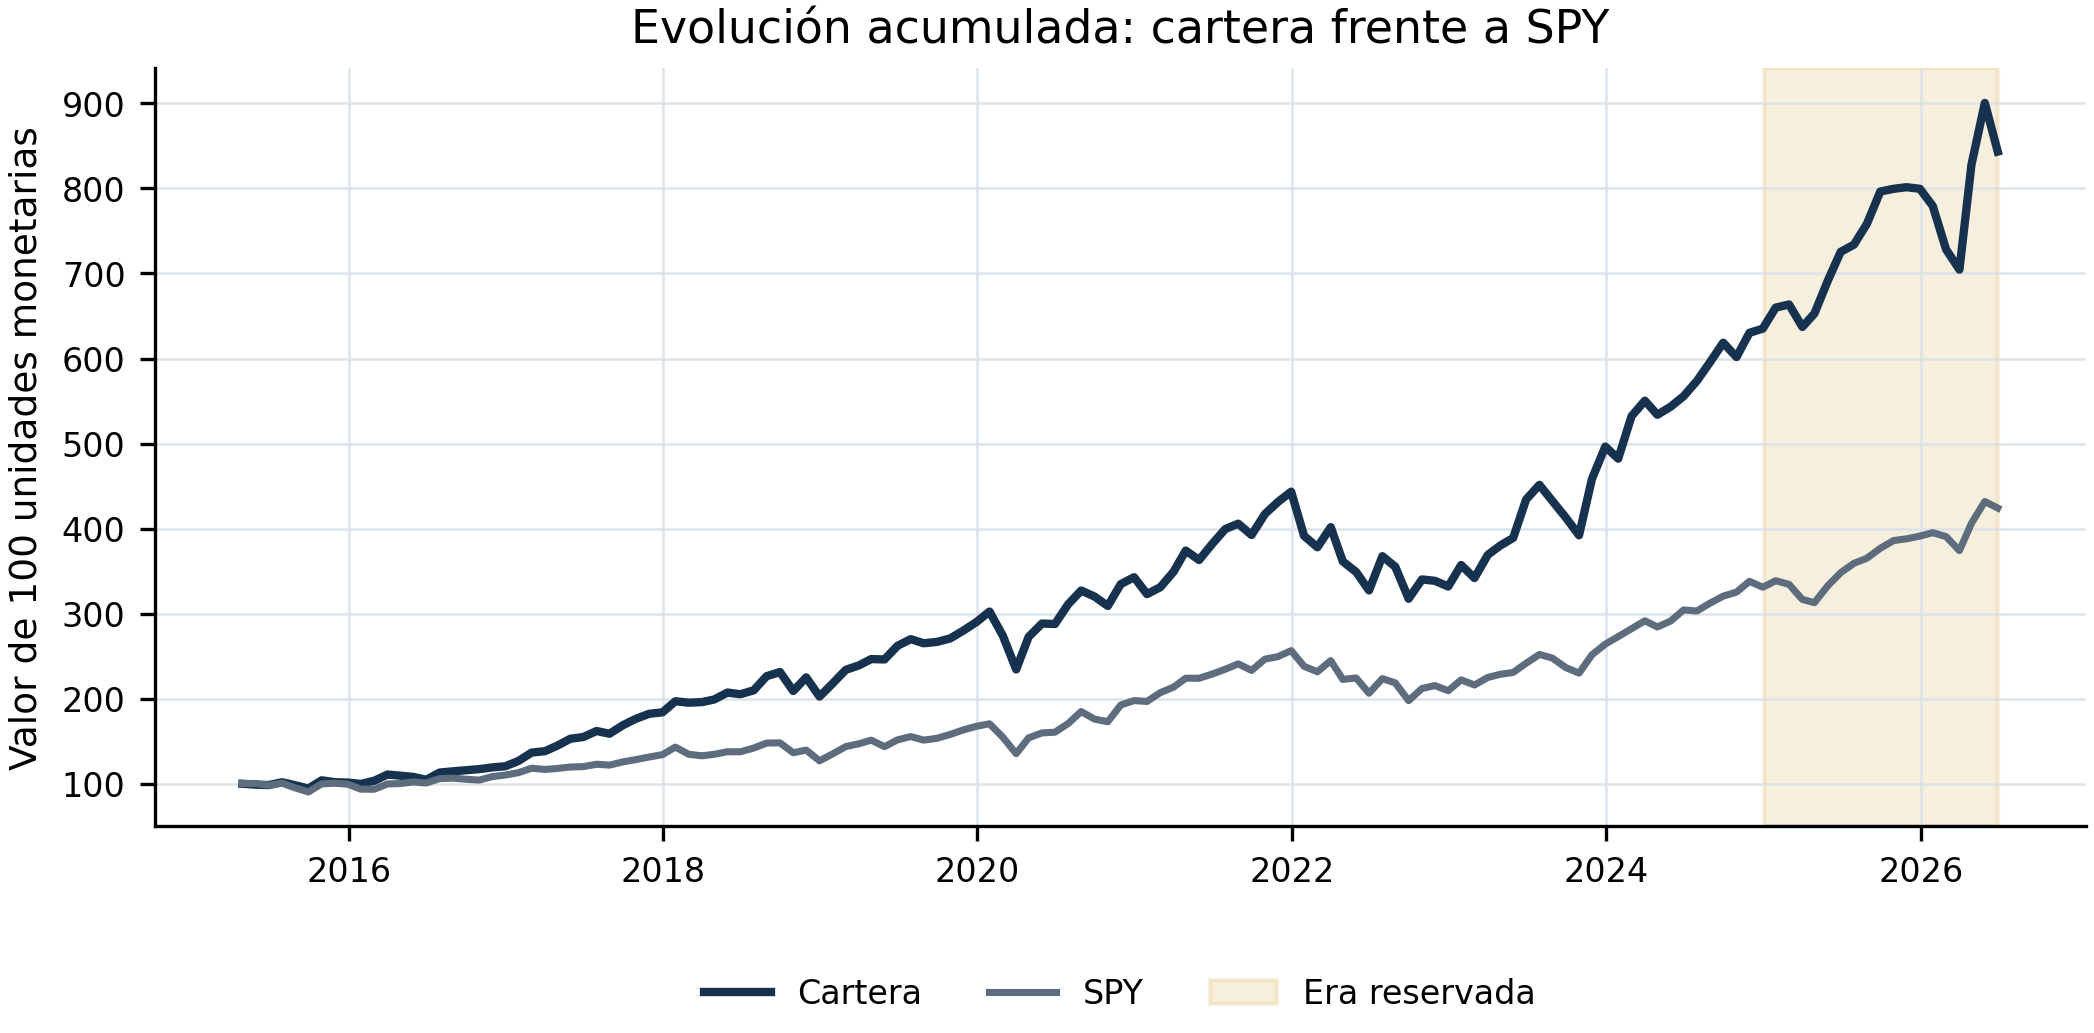
\includegraphics[width=0.96\textwidth]{assets/f07_equity.png}
  \caption{Curva de patrimonio de la cartera y SPY. La región dorada es confirmación reservada,
  no selección. Fuente: \texttt{evidence/equity.parquet}.}
  \label{fig:equity}
\end{figure}

\begin{figure}[H]
  \centering
  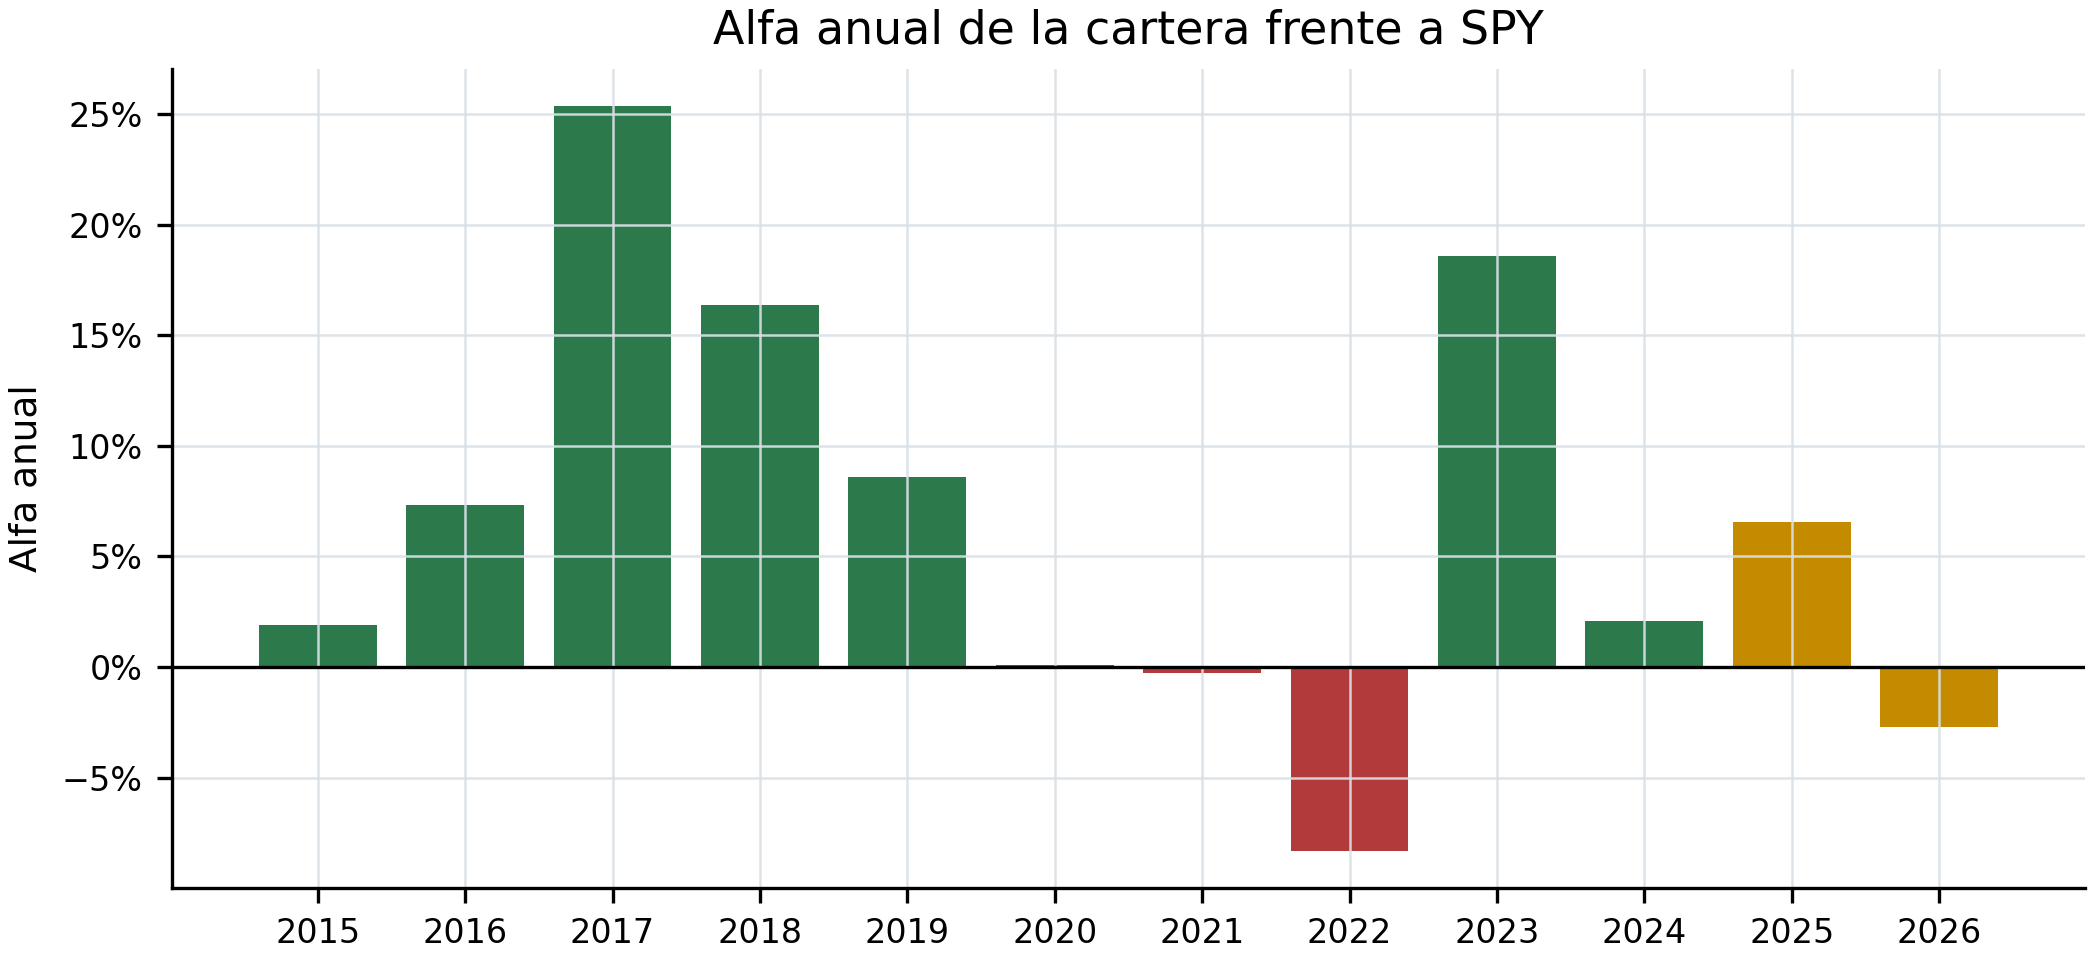
\includegraphics[width=0.91\textwidth]{assets/f07_alfa_anual.png}
  \caption{Alfa anual. El color dorado marca 2025--2026. Fuente:
  \texttt{evidence/annual\_metrics.parquet}.}
  \label{fig:alfa-anual}
\end{figure}

\begin{table}[H]
  \centering
  \scriptsize
  \caption{Resultado anual de la cartera.}
  \label{tab:anual}
  \begin{tabular}{lrrrrrrr}
\toprule
Año & Cartera & SPY & Alfa & MDD & IR & Efectivo & Turnover \\
\midrule
2015 & 1,27\% & -0,63\% & 1,91\% & 7,30\% & 0,434 & 0,00\% & 158,59\% \\
2016 & 19,00\% & 10,88\% & 7,32\% & 5,59\% & 0,814 & 0,00\% & 379,81\% \\
2017 & 52,56\% & 21,71\% & 25,35\% & 1,98\% & 3,877 & 0,00\% & 308,32\% \\
2018 & 10,10\% & -5,40\% & 16,38\% & 12,50\% & 1,887 & 0,00\% & 291,11\% \\
2019 & 43,38\% & 32,05\% & 8,57\% & 1,80\% & 1,553 & 0,00\% & 332,78\% \\
2020 & 18,13\% & 18,02\% & 0,09\% & 22,52\% & 0,067 & 0,00\% & 361,61\% \\
2021 & 29,34\% & 29,71\% & -0,29\% & 3,28\% & 0,032 & 0,00\% & 265,83\% \\
2022 & -25,16\% & -18,38\% & -8,30\% & 20,96\% & -0,928 & 0,00\% & 120,14\% \\
2023 & 49,61\% & 26,18\% & 18,57\% & 13,14\% & 1,679 & 0,00\% & 468,60\% \\
2024 & 27,94\% & 25,34\% & 2,07\% & 3,01\% & 0,213 & 0,00\% & 476,39\% \\
2025 & 25,90\% & 18,17\% & 6,55\% & 3,99\% & 1,056 & 0,00\% & 330,53\% \\
2026 & 5,48\% & 8,43\% & -2,73\% & 9,60\% & -0,123 & 0,00\% & 256,49\% \\
\bottomrule
\end{tabular}

  \caption*{Fuente: \texttt{evidence/annual\_metrics.parquet}. Turnover anualizado; efectivo medio.}
\end{table}

La era reservada 2025--2026 ofrece una confirmación económica positiva, pero que sólo se sostiene
con la cartera optimizada. Con ella, el CAGR de cartera es 22,23\% frente a 19,18\% de SPY, el
exceso geométrico 2,56\%, el IR 0,304 y se bate al índice en uno de los dos años, con un turnover
anualizado de 391,35\%. Con la cartera por defecto del Model Study, la misma señal producía en esa
misma era un exceso de $-11,29$\%, un IR de $-1,167$ y ningún año por encima del índice. La
diferencia entre ambos resultados no procede del modelo, que es idéntico, sino de la construcción
de cartera, y es la razón por la que este trabajo dedica un estudio entero a esa construcción.

El Rank-IC de la era reservada es $+0,0441$ sobre seis cohortes, con 66,67\% de ellas positivas.
Es positivo, aunque inferior al 0,1090 de la ventana de selección, y descansa sobre
aproximadamente una observación independiente efectiva. No debe leerse como confirmación predictiva
concluyente sino como indicio compatible con el resto de la evidencia: la ordenación no se rompió
fuera de la ventana de decisión, se debilitó.

Una precisión sobre las fuentes es necesaria para no atribuir a la cartera optimizada una cifra que
no le corresponde. El alfa factorial de la era reservada que persiste \artefacto{attribution.json}
--- con $t=-3,50$ --- se calculó sobre la cartera del Model Study, no sobre la ganadora de la
rejilla, porque la atribución factorial forma parte de la evidencia predictiva y se computa antes de
optimizar la cartera. Ese estadístico documenta, por tanto, hasta qué punto la cartera \emph{por
defecto} destruía valor en esa era, y no debe citarse como veredicto sobre la cartera finalmente
adoptada.

\begin{figure}[H]
  \centering
  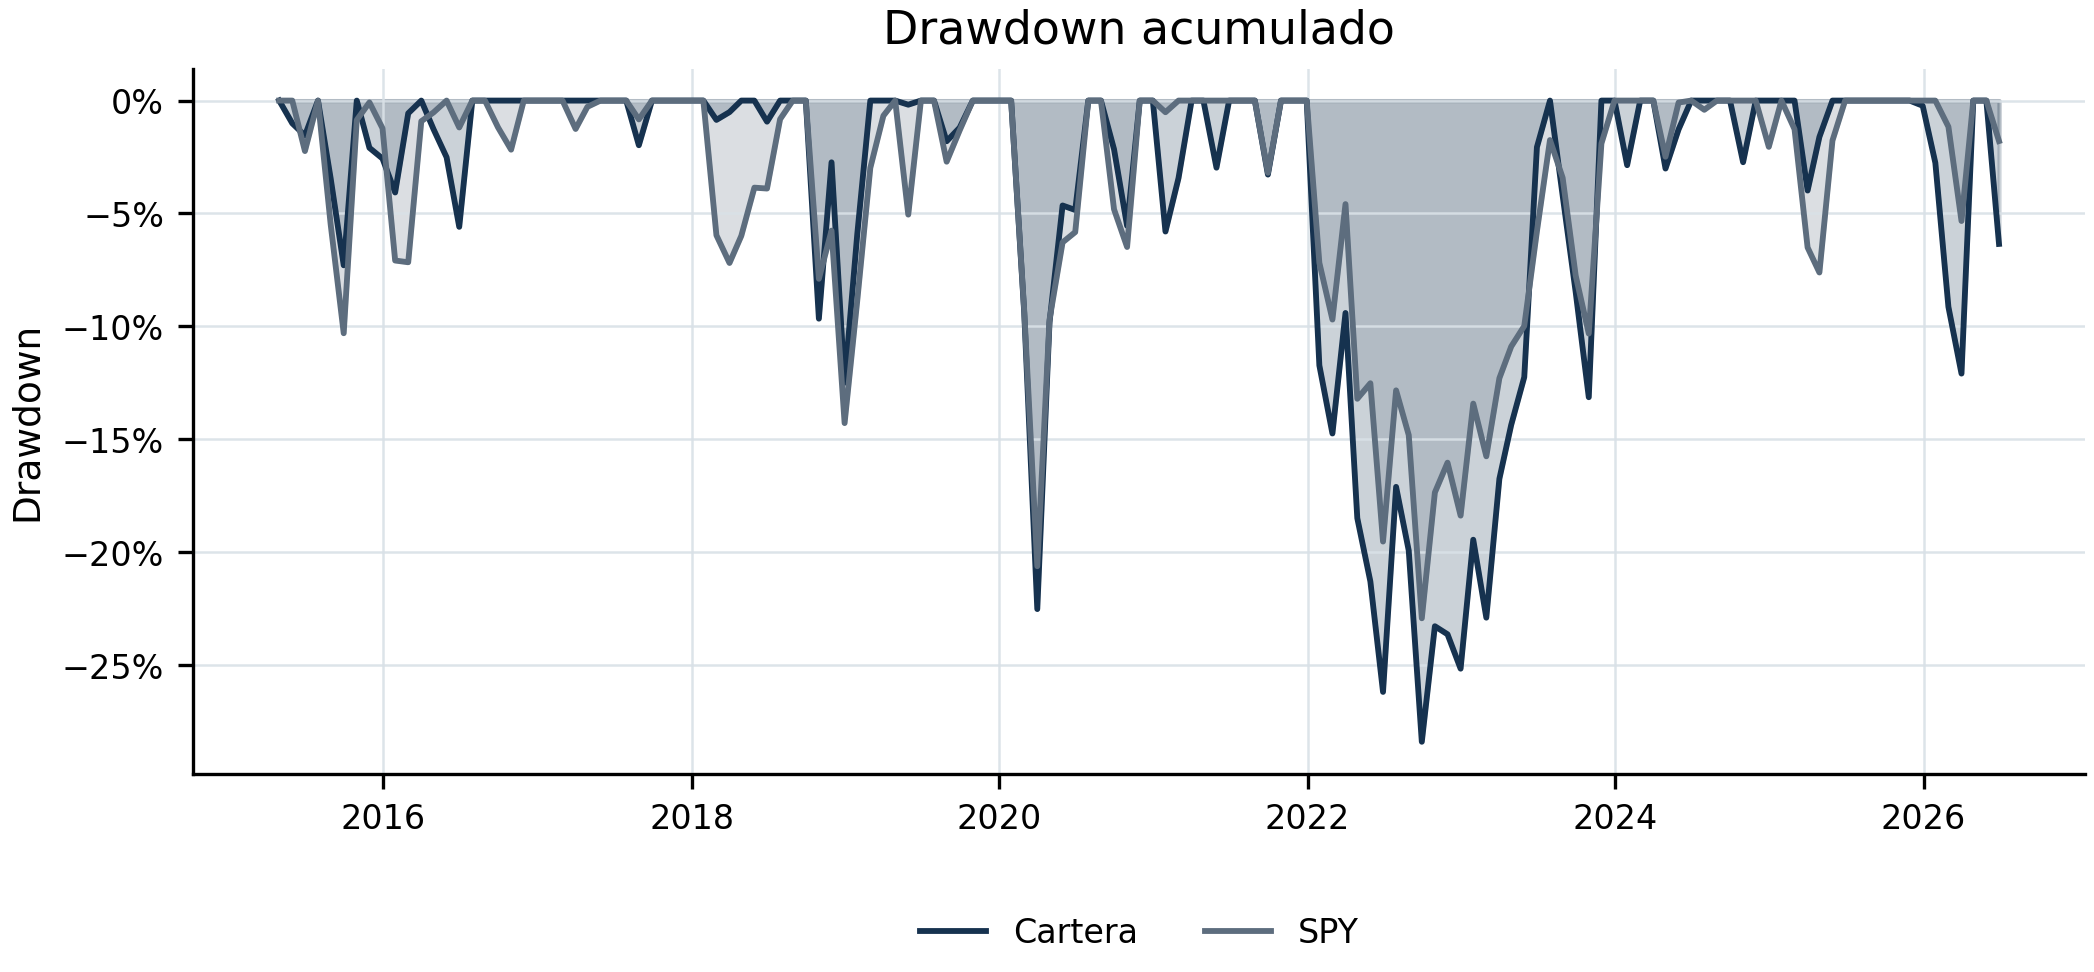
\includegraphics[width=0.92\textwidth]{assets/f07_drawdown.png}
  \caption{Drawdown acumulado de cartera y SPY. Fuente: \texttt{evidence/equity.parquet}.}
  \label{fig:drawdown}
\end{figure}

\section{Perfiles y coeficiente de transferencia}

Los ocho perfiles comparten el mismo Rank-IC; sólo modifican la manera de llevarlo a cartera. Es un
experimento controlado: las diferencias no pueden atribuirse a otro modelo. \texttt{balanced}, que
no reordena la señal del meta, alcanza el mayor IR y el mayor exceso geométrico. Seis de los siete
perfiles que imponen un sesgo adicional destruyen alfa; \texttt{momentum} es el peor, con el mayor
turnover.

Las cifras de los perfiles se presentan una sola vez, con la cartera ganadora, en la
Sección~\ref{sec:cartera-rejilla}. Evaluarlos también con la cartera del Model Study daría dos
valores distintos para el mismo perfil --- y un ganador distinto --- sin añadir nada: lo que
interesa es cómo se comporta cada estilo con la gestión que el trabajo adopta.

\begin{figure}[H]
  \centering
  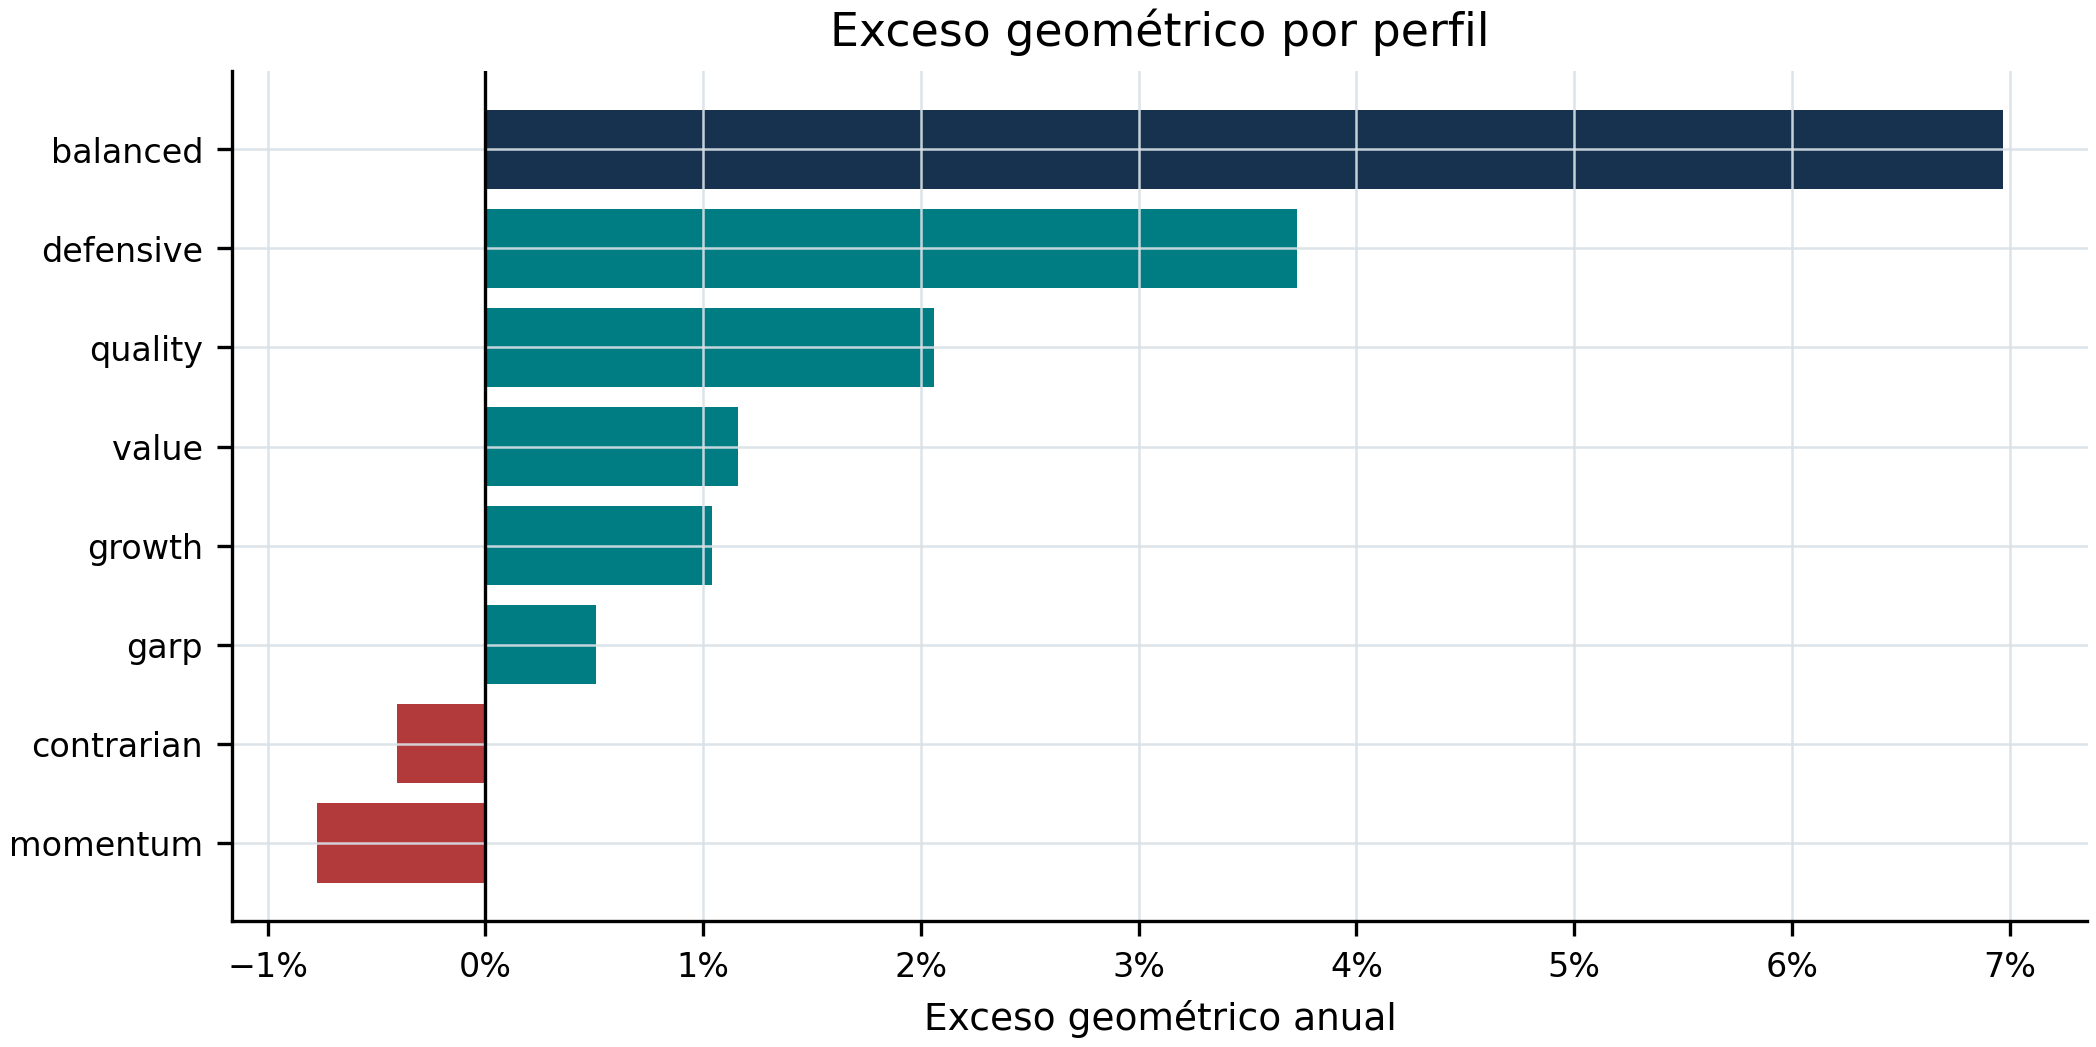
\includegraphics[width=0.90\textwidth]{assets/f07_perfiles_exceso.png}
  \caption{Exceso geométrico por perfil, con la cartera ganadora. Fuente:
  \artefacto{portfolio\_profiles.parquet}.}
  \label{fig:perfiles-exceso}
\end{figure}

El coeficiente de transferencia de la cartera del Model Study es 0,328: materializa aproximadamente
un tercio de la señal disponible. La ley fundamental de la gestión activa relaciona IR, IC, amplitud
y transferencia; en este caso la restricción \textit{long-only}, el número de nombres, el coste de
transacción y una rotación superior al 300\% explican que la limitación práctica esté en la cartera
y no necesariamente en el ranking. Esta lectura concuerda con la distinción entre calidad de señal e
implementación de López de Prado (2018).

Merece subrayarse que la transferencia mejoró de forma sostenida a lo largo de la cadena --- 0,178,
0,234 y 0,328 ---, es decir, que cada pasada no sólo ordenó algo mejor sino que además consiguió
llevar a la cartera una fracción mayor de lo que ordenaba. Y el Portfolio Study puede leerse como la
continuación natural de esa misma línea: si la limitación estaba en la implementación, atacarla
directamente era la palanca disponible, y el resultado de la Sección~\ref{sec:cartera-rejilla}
confirma que lo era.

\begin{figure}[H]
  \centering
  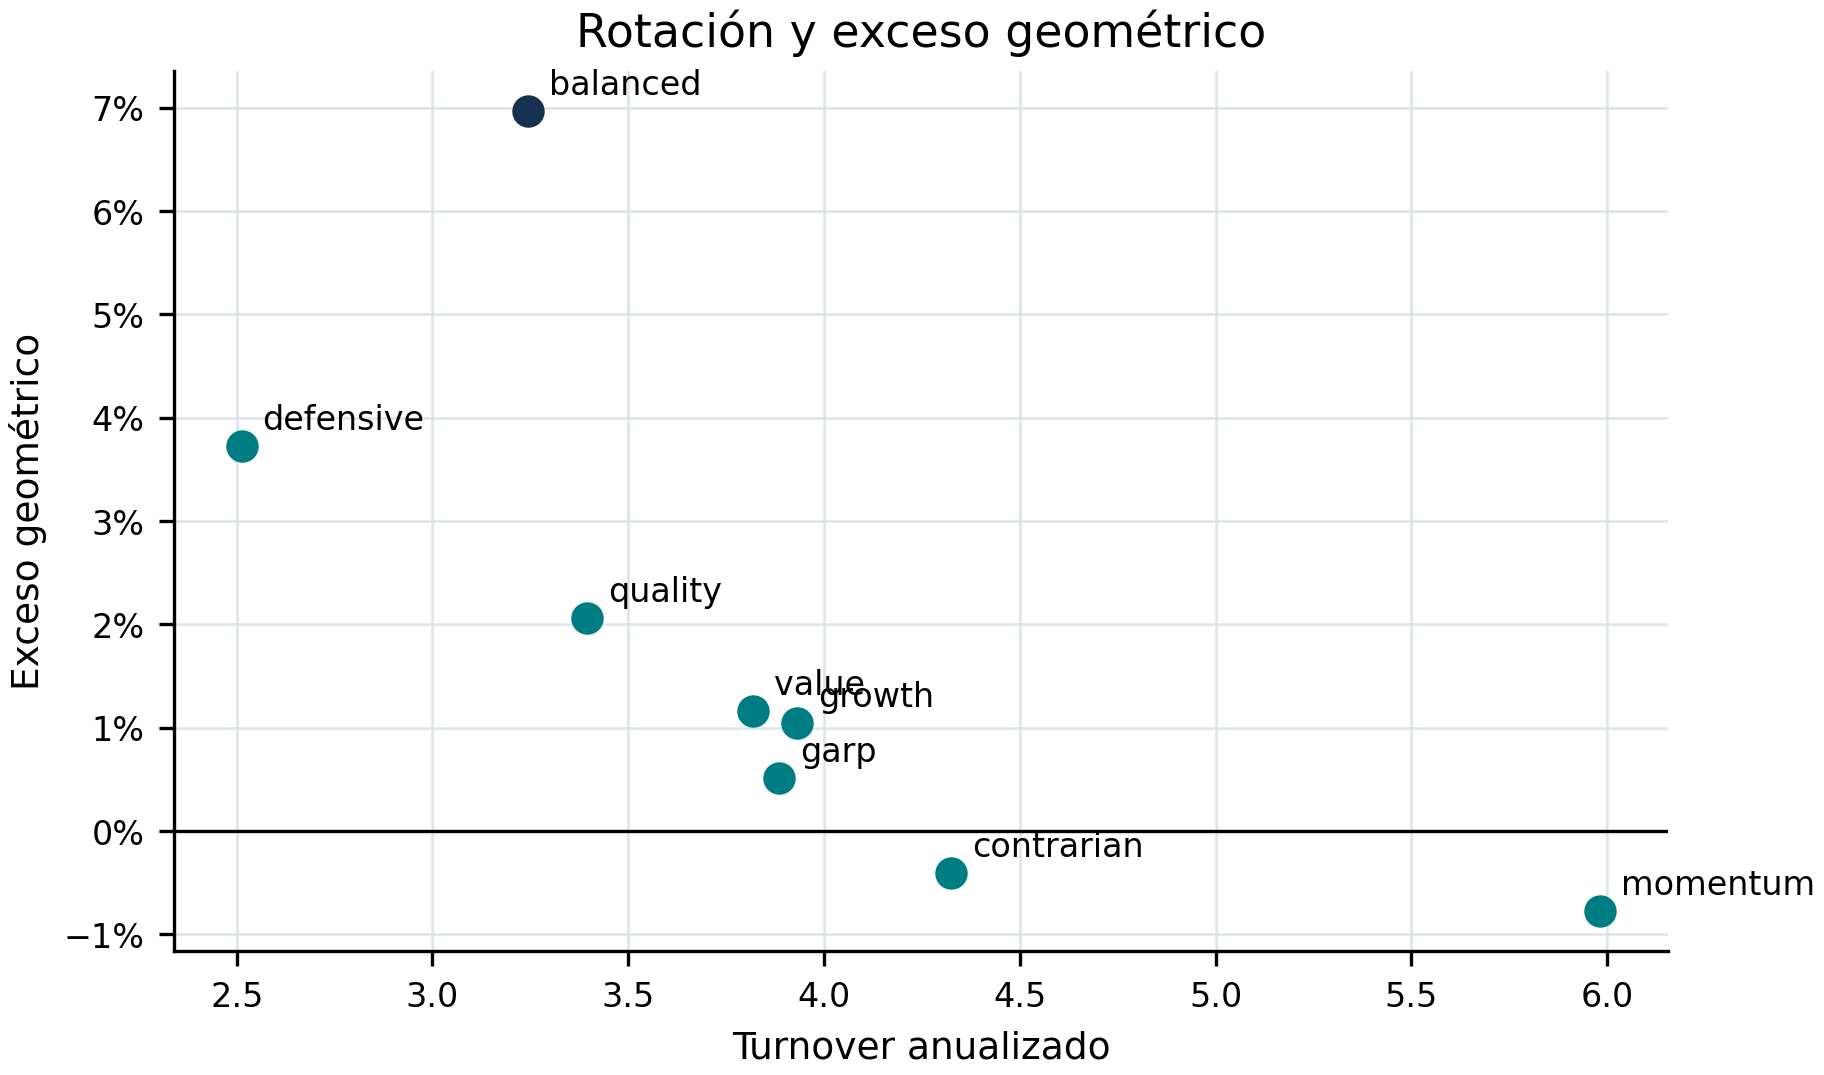
\includegraphics[width=0.84\textwidth]{assets/f07_perfiles_tradeoff.png}
\caption{Relación entre rotación y exceso geométrico de los perfiles, con la cartera ganadora.
Fuente: \artefacto{portfolio\_profiles.parquet}.}
\label{fig:perfiles-tradeoff}
\end{figure}

\section{Lectura conjunta de la evidencia}

Los resultados no deben reducirse a la frase ``la cartera batió al índice''. La evidencia tiene tres
capas y cada una contesta una pregunta distinta. La primera es predictiva: el Rank-IC indica que el
orden transversal contiene información y que el sistema supera los baselines deterministas. La
segunda es estadística: permutación, placebos, bootstrap, exclusión de eras y semillas evalúan si la
relación podría ser azar, un defecto mecánico o una coincidencia de régimen. La tercera es económica:
la cartera muestra qué parte de esa señal sobrevive a restricciones long-only, costes y tamaño
limitado. Con esa secuencia en mente, la sección siguiente traduce la señal ya validada a resultado
de cartera.

\section{Atribución, factores y resultado no superado}

La neutralización de estilo reduce el Rank-IC de 0,1177 a 0,1019. La pérdida del 13,38\% indica que
parte de la señal comparte información con controles conocidos, como sería esperable en un sistema
que utiliza ratios económicos y medidas de riesgo. La retención del 86,62\% muestra, sin embargo,
que no se agota en esos controles. La regresión factorial tiene $R^2=0,017$ y no presenta cargas
significativas, pero el alfa de selección tampoco es significativo de forma aislada. La conclusión
prudente es que la evidencia es compatible con una señal parcialmente distinta de los factores
implementados, no que haya descubierto una prima nueva y causal.

\begin{table}[H]
  \centering
  \small
  \caption{Neutralización del Rank-IC por controles de estilo.}
  \label{tab:neutralizacion}
  \begin{tabular}{lr}
\toprule
Concepto & Valor \\
\midrule
Rank-IC bruto & 0,1177 \\
Rank-IC neutralizado & 0,1019 \\
Fracción retenida & 86,62\% \\
Controles aplicados & 14 \\
Cohortes & 117 \\
\bottomrule
\end{tabular}

  \caption*{Fuente: \artefacto{attribution.json}. Los catorce controles son ratios de valoración,
  rentabilidad, crecimiento, volatilidad y beta, listados en el Anexo~\ref{anexo:evidencia}.}
\end{table}

La regresión factorial merece un examen por ventanas, porque su lectura cambia radicalmente entre
ellas y esa diferencia es en sí misma un resultado. La Tabla~\ref{tab:factores} y la
Figura~\ref{fig:factores} la presentan.

\begin{table}[H]
  \centering
  \scriptsize
  \caption{Regresión factorial con errores Newey--West de doce retardos, por ventana.}
  \label{tab:factores}
  \begin{tabular}{lrrrrrrrrr}
\toprule
Ventana & Alfa/periodo & $t$ & $R^2$ & Obs. & value & momentum & low volatility & quality & growth \\
\midrule
Selección & 0,27\% & 1,44 & 0,017 & 117 & 0,003 & -0,105 & 0,070 & 0,056 & 0,062 \\
Confirmación & -0,48\% & -3,50 & 0,341 & 17 & -0,346 & 0,029 & -0,116 & -0,219 & -0,247 \\
Curva completa & 0,19\% & 1,06 & 0,011 & 134 & -0,039 & -0,069 & 0,025 & 0,025 & 0,063 \\
\bottomrule
\end{tabular}

  \caption*{Calculado sobre la cartera del Model Study: la atribución factorial forma parte de la
  evidencia predictiva y se computa antes de optimizar la cartera. No describe, por tanto, a la
  cartera finalmente adoptada.}
  \caption*{Fuente: \artefacto{attribution.json}. Los factores de tamaño e inversión no son
  construibles con las fuentes disponibles y se declaran no replicables en lugar de sustituirse por
  un sucedáneo no auditable.}
\end{table}

\begin{figure}[H]
  \centering
  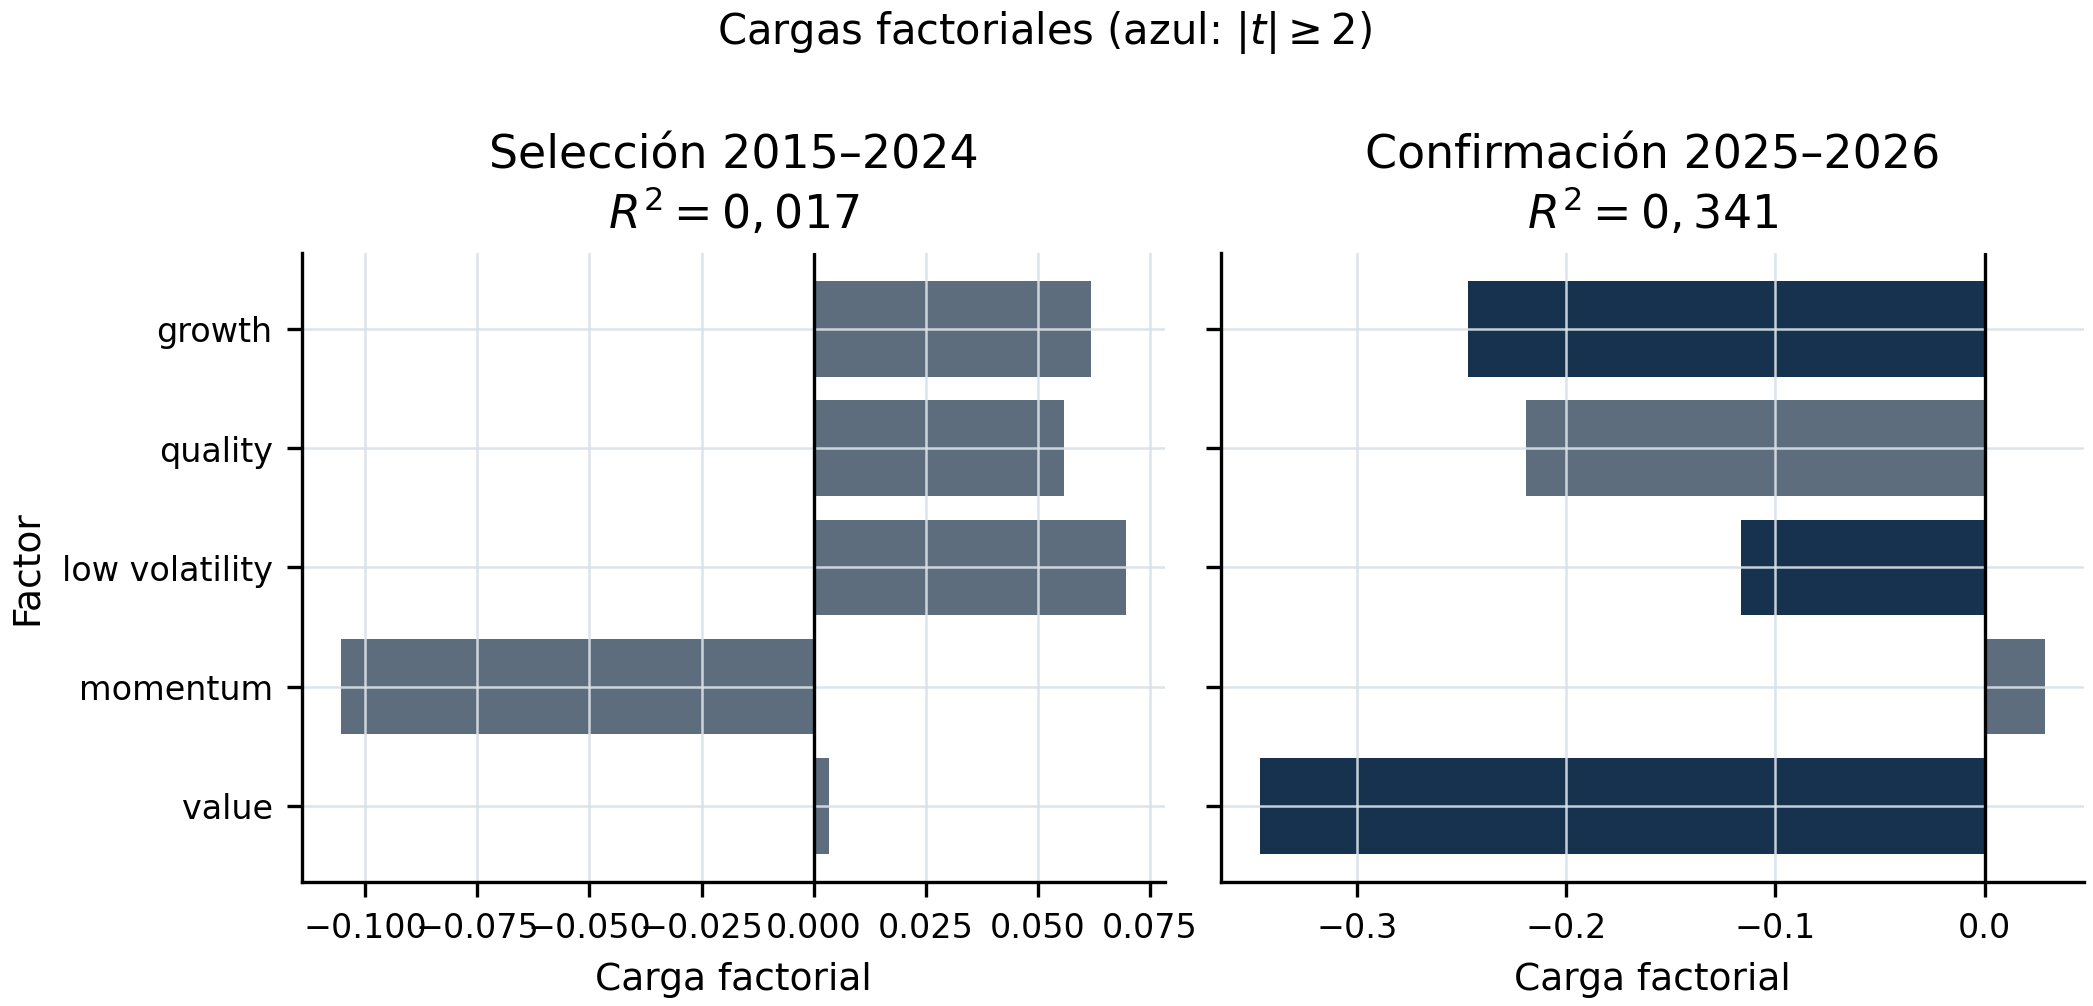
\includegraphics[width=0.94\textwidth]{assets/f07_factores.png}
  \caption{Cargas factoriales en las ventanas de selección y confirmación. En azul, las cargas con
  $|t|\geq 2$. Fuente: \artefacto{attribution.json}.}
  \label{fig:factores}
\end{figure}

En la ventana de selección el modelo apenas tiene estructura factorial: $R^2=0,019$ y ninguna carga
significativa. En la de confirmación, en cambio, $R^2=0,447$ y aparecen cargas grandes y
significativas --- negativa en valor y en calidad, positiva en crecimiento y en baja volatilidad ---
junto a un alfa por periodo de 0,84\,\% con $t=2,53$. La tentación sería presentar únicamente el
alfa significativo de la era reservada. Sería un error de lectura: con diecisiete observaciones y
cinco regresores, un $R^2$ de 0,447 es exactamente lo que cabe esperar por construcción, y las
cargas no describen tanto una exposición estable como el hecho de que dos años concretos tuvieron
un carácter factorial marcado. La conclusión defendible es la conservadora: el sistema no muestra
una exposición factorial estable a lo largo del tiempo, y su alfa no puede declararse
significativo en la ventana donde se dispone de potencia estadística.

El Deflated Sharpe de 0,682, inferior a 0,95, es la limitación empírica más importante, y su valor
ha empeorado respecto de las pasadas anteriores de la cadena precisamente porque la cadena existe:
el estadístico penaliza el Sharpe por el número de configuraciones ensayadas, y encadenar estudios
multiplica ese número. Recuerda, por tanto, que una rentabilidad histórica seleccionada entre
decenas de alternativas merece escepticismo adicional. No contradice el test de permutación del
Rank-IC: ambos examinan objetos diferentes. El primero limita una afirmación de rentabilidad
ajustada por riesgo; el segundo apoya que el ranking no se comporta como ruido puro. Que uno se
debilite mientras el otro se mantiene es exactamente el patrón esperable cuando se busca más: la
evidencia de \emph{señal} resiste y la de \emph{rentabilidad} se encarece.

\section{Análisis de los años adversos y de la era reservada}

Los años con alfa negativo de la ventana de selección, 2021 y 2022, son informativos. En 2021 la
cartera quedó a 0,29 puntos porcentuales del índice, una diferencia que no requiere explicación
estructural. En 2022, en cambio, perdió 8,30 puntos en un año de caída generalizada, y lo hizo con
la rotación más baja de toda la serie (1,20): no fue un problema de fricción sino de composición,
lo que resulta coherente con un sistema que ordena por atractivo relativo y no gestiona la
exposición direccional al mercado.

Es una limitación real de diseño, y conviene enunciarla como tal: el sistema decide \emph{qué}
comprar, no \emph{cuánto} estar expuesto. La política de efectivo es lo más parecido a una palanca
de exposición que tiene, y la cartera ganadora la fija en cero. El resultado es una cartera que
participa íntegramente de las caídas del mercado y aspira a superarlas en términos relativos, no a
evitarlas.

La era reservada ofrece el contraste decisivo del trabajo, y su lectura depende por completo de qué
cartera se use para materializar la señal. Con la cartera optimizada, el exceso geométrico de
2,56\%, el IR de 0,304 y un año de dos por encima de SPY son económicamente positivos y no pudieron
intervenir en ninguna elección. Con la cartera por defecto, la misma señal daba $-11,29$\% e IR
$-1,167$. El Rank-IC de la era, $+0,0441$, es positivo en ambos casos porque no depende de la
cartera: es la señal, y la señal se sostuvo.

Se informa junto a su debilidad estadística, que es considerable: sólo seis cohortes tienen etiqueta
cerrada, varias observaciones futuras no han madurado y el número independiente efectivo es
aproximadamente uno. El trabajo no convierte esa combinación en una demostración. Lo que afirma es
más modesto y más defendible: en la única ventana que no participó en ninguna decisión, la
ordenación aprendida siguió siendo positiva, y su traducción a rentabilidad dependió de la
construcción de cartera hasta el punto de cambiar de signo.

\section{Gestión de cartera: la rejilla completa}
\label{sec:cartera-rejilla}

Las variables de cartera del catálogo no son predictivas: se ejecutan \emph{después} de congelar el
ganador y nunca influyen en su selección. Esa separación, impuesta por el protocolo, tiene una
consecuencia metodológica valiosa. Como todas las carteras parten exactamente del mismo modelo, de
la misma señal y del mismo panel, sus diferencias sólo pueden atribuirse a la regla de construcción
de cartera. Es un experimento controlado en sentido estricto.

Una versión anterior de este trabajo exploraba esas reglas de una en una, cambiando una variable
sobre la configuración recomendada y dejando las demás fijas. Ese barrido diagnóstico producía un
resultado incómodo --- buena parte de las variantes batían a la cartera empleada --- que el
documento se limitaba a reportar sin actuar, porque cambiar el ganador a la vista de su rentabilidad
conocida es exactamente lo que el protocolo prohíbe. El Capítulo~\ref{chap:desarrollo-cartera}
explica por qué esa renuncia era innecesaria y cómo se sustituye por una optimización legítima: se
recorre el producto cartesiano de las seis variables que gobiernan la cartera, se optimiza el
Information Ratio en lugar del exceso bruto, y \textbf{la rejilla se calcula sobre una serie
recortada en 2024}, de modo que ninguna de las combinaciones evaluadas puede ver la era reservada.
No es que se ignore su resultado: es que no llega a calcularse.

\begin{table}[H]
  \centering
  \small
  \caption{Cuánto separa cada variable de cartera el Information Ratio.}
  \label{tab:cartera-influencia}
  \begin{tabular}{llrlrr}
\toprule
Variable & Mejor valor & IR mediano & Peor valor & IR mediano & Diferencia \\
\midrule
Posiciones objetivo & 5 & 0,461 & 50 & 0,160 & 0,300 \\
Tope de efectivo & 0.0 & 0,360 & 0.25 & 0,158 & 0,202 \\
Suelo de cobertura & 0.0 & 0,341 & 80.0 & 0,234 & 0,107 \\
Tenencia mínima & none & 0,325 & full horizon & 0,286 & 0,039 \\
Tolerancia de deriva & 0.1 & 0,314 & 0.4 & 0,298 & 0,016 \\
Reparto de pesos & alpha proportional & 0,312 & equal & 0,303 & 0,009 \\
\bottomrule
\end{tabular}

  \caption*{Fuente: \artefacto{portfolio\_grid.parquet}. Para cada variable se toma la mediana del
  IR de todas las carteras que comparten un valor, con las otras cinco variando libremente, y se
  comparan el mejor y el peor valor. No se tabulan las mejores carteras individuales porque se
  diferencian en un decimal y repiten la misma configuración con variaciones menores.}
\end{table}

La Tabla~\ref{tab:cartera-influencia} ordena las seis variables por cuánto importan, y el resultado
es desigual. Las dos que gobiernan la exposición separan el Information Ratio de forma decisiva
--- 0,300 el número de posiciones y 0,202 el tope de efectivo ---, el suelo de cobertura aporta
0,107, y las tres restantes se mueven por debajo de 0,04. En particular, el reparto de pesos (0,009)
y la tolerancia de deriva (0,016) son, a efectos del IR, prácticamente indiferentes.

Hay en esa tabla un argumento a favor del método que conviene explicitar. Si se eligiera cada
variable por su mejor valor marginal, el número de posiciones sería \textbf{5}, que es el que
maximiza la mediana. La cartera ganadora usa \textbf{8}. No es una contradicción: la mediana marginal
promedia sobre todas las combinaciones de las otras cinco variables, mientras que la ganadora es un
punto concreto donde esas cinco toman valores concretos. Dicho de otro modo, \emph{optimizar variable
a variable no habría encontrado la cartera ganadora}, que es exactamente la razón por la que esta
búsqueda es cartesiana y no secuencial, como se argumenta en el
Capítulo~\ref{chap:desarrollo-cartera}.

\begin{figure}[H]
  \centering
  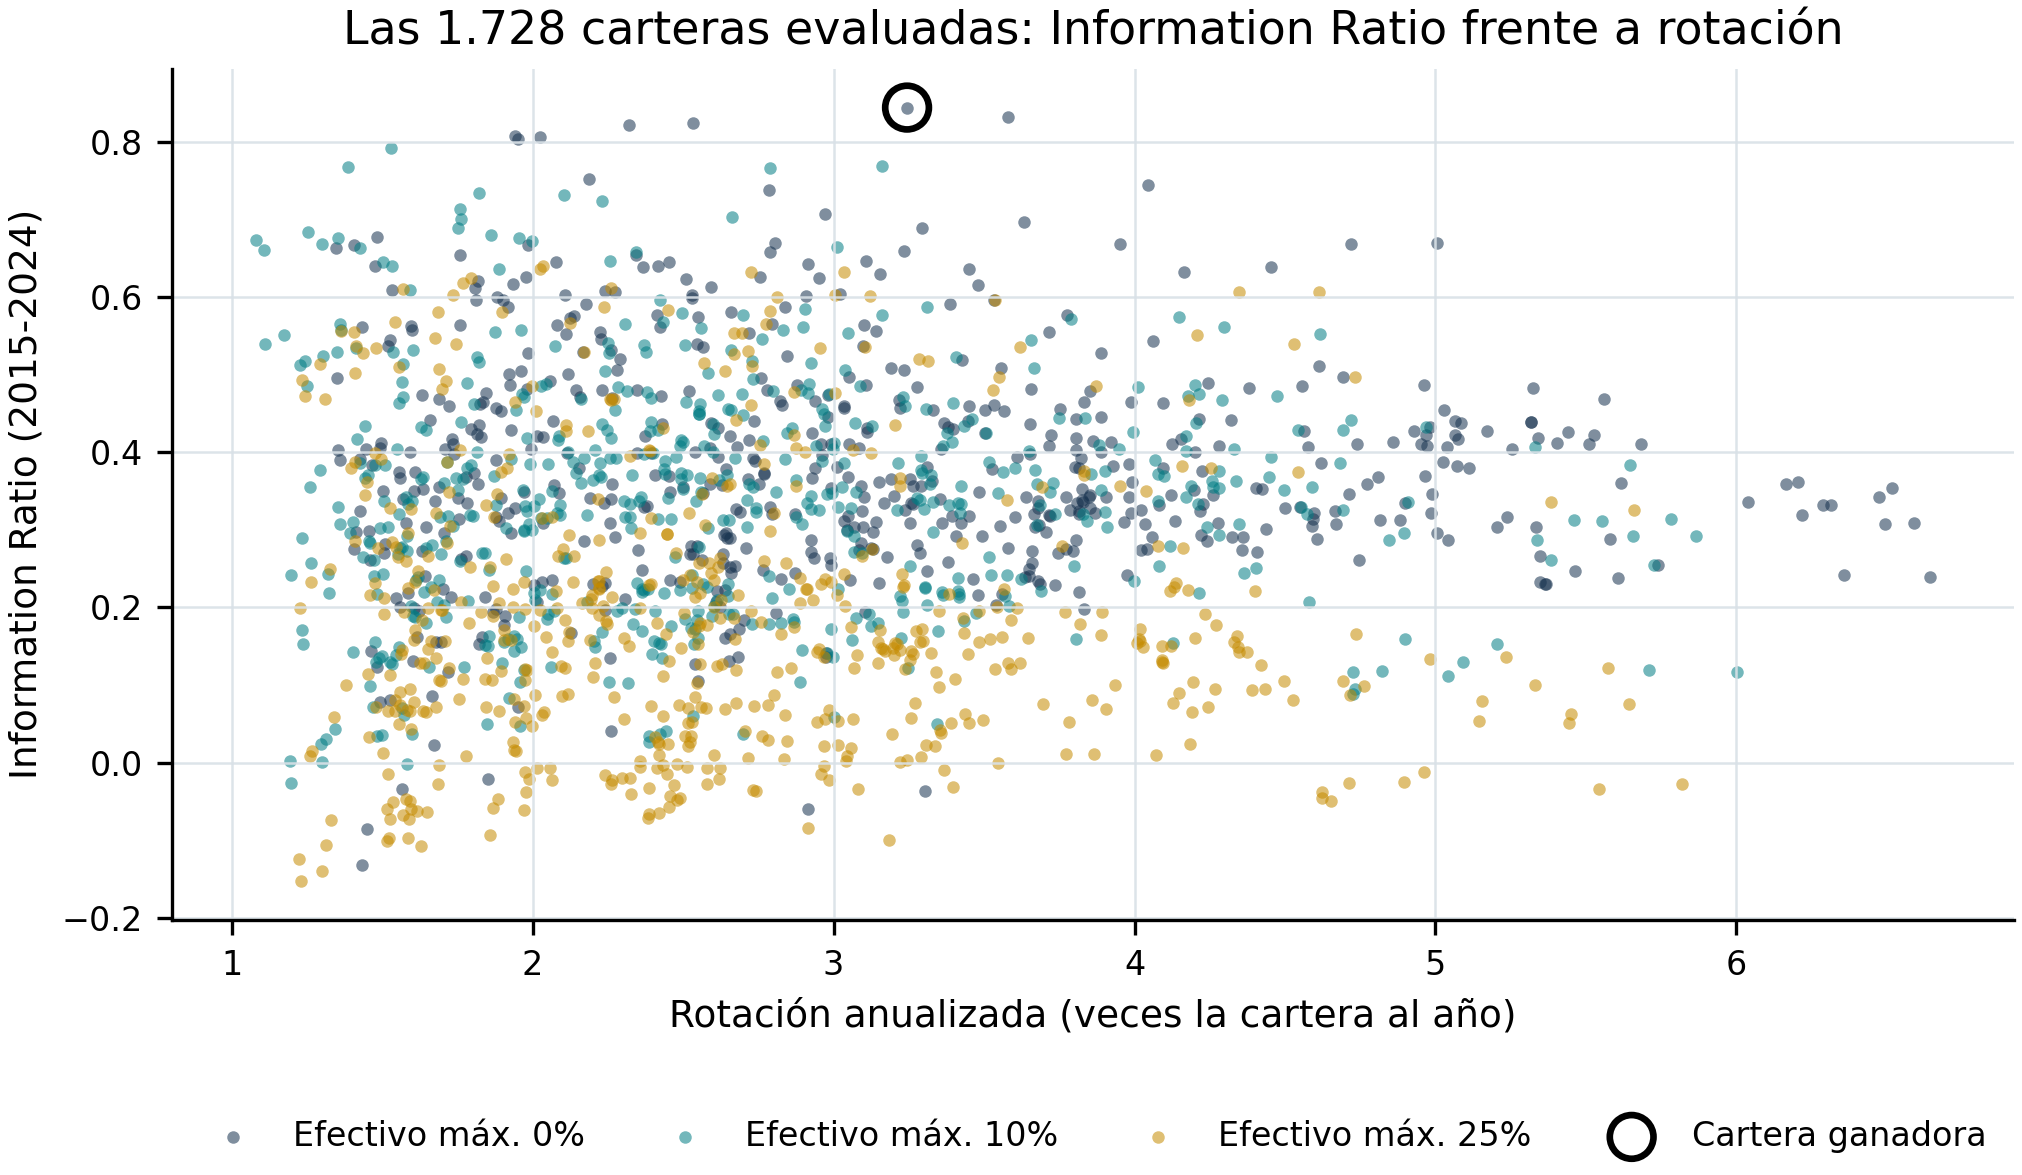
\includegraphics[width=0.94\textwidth]{assets/f08_cartera_rejilla.png}
  \caption{Las carteras evaluadas en el plano rotación--Information Ratio. Cada punto es una cartera
  completa, con las seis coordenadas fijadas a la vez; el color codifica el tope de efectivo y el
  círculo negro señala la ganadora. Fuente: \artefacto{portfolio\_grid.parquet}.}
  \label{fig:cartera-rejilla}
\end{figure}

La nube de la Figura~\ref{fig:cartera-rejilla} deja ver de entrada que el Information Ratio no es
una función de la rotación: para casi cualquier nivel de turnover existen carteras buenas y
carteras mediocres, de modo que rotar poco no es en sí mismo una virtud ni rotar mucho un defecto.
Lo que sí separa la nube con claridad es el tope de efectivo, cuya banda superior se agrupa en los
topes bajos.

\begin{figure}[H]
  \centering
  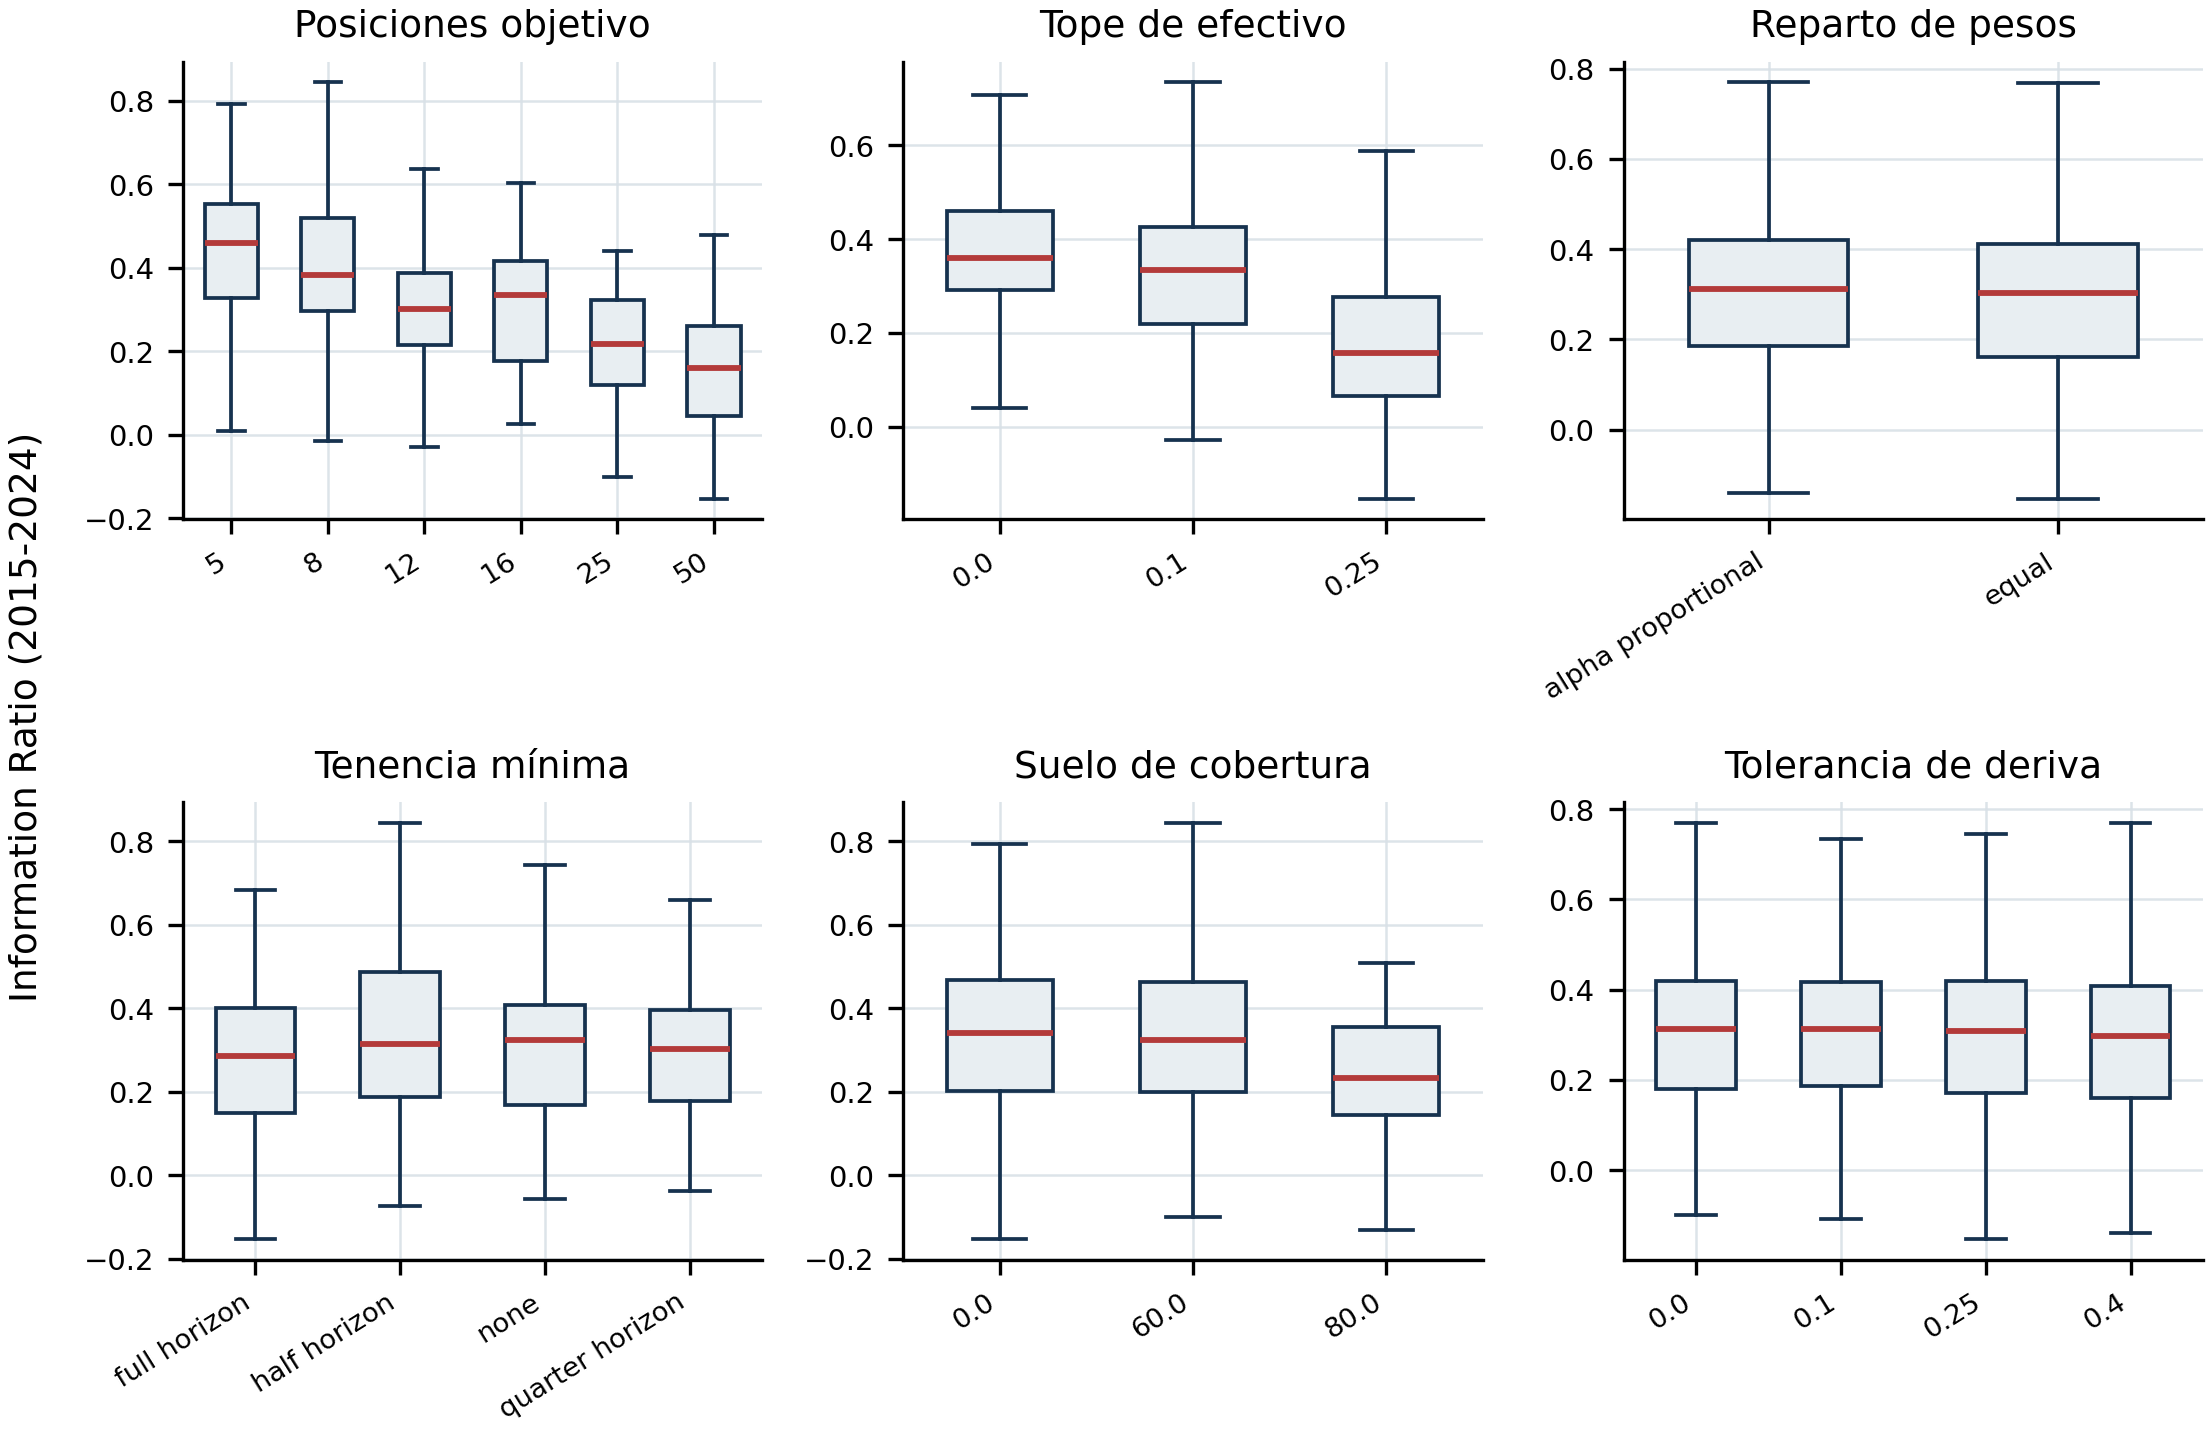
\includegraphics[width=0.96\textwidth]{assets/f08_cartera_marginales.png}
  \caption{Efecto marginal de cada variable sobre el Information Ratio. Cada caja resume todas las
  carteras que comparten ese valor, con las cinco variables restantes variando libremente. Fuente:
  \artefacto{portfolio\_grid.parquet}.}
  \label{fig:cartera-marginales}
\end{figure}

La Figura~\ref{fig:cartera-marginales} ordena las seis variables por cuánto importan, y el resultado
corrige la intuición de partida. Las dos que gobiernan la exposición --- el número de posiciones y
el tope de efectivo --- desplazan la distribución del IR de forma inequívoca, mientras que la
tolerancia de deriva apenas la mueve: sus cuatro cajas son casi indistinguibles, lo que significa
que esa variable es, a efectos del Information Ratio, prácticamente inerte. Es una conclusión que el
barrido de una variable cada vez no podía alcanzar, porque no distinguía entre «este valor es
mejor» y «esta variable da igual».

Estas cajas admiten una única lectura honesta, y conviene enunciarla antes de sacar conclusiones:
al fijar una coordenada, las otras cinco siguen variando, de modo que cada caja resume un
\emph{conjunto} de carteras y no una cartera concreta. Una mediana alta indica que ese valor tiende
a funcionar bien acompañado de casi cualquier cosa, no que baste con adoptarlo.

\subsection*{La cartera ganadora}

\begin{table}[H]
  \centering
  \caption{Configuración de cartera ganadora de la rejilla.}
  \label{tab:cartera-ganadora-config}
  \begin{tabular}{ll}
\toprule
Variable de cartera & Valor ganador \\
\midrule
Posiciones objetivo & 8 \\
Tope de efectivo & 0.0 \\
Reparto de pesos & alpha proportional \\
Tenencia mínima & half horizon \\
Suelo de cobertura & 60.0 \\
Tolerancia de deriva & 0.1 \\
\bottomrule
\end{tabular}

  \caption*{Fuente: \artefacto{portfolio\_winner.json}, campo \texttt{winner\_combination}.}
\end{table}

La cartera elegida concentra en ocho posiciones, reparte el peso en proporción al alfa esperado, no
sostiene efectivo, retiene cada posición al menos medio horizonte, corta por debajo del percentil 60
y corrige la deriva al 10\,\%. Es una cartera \emph{más} concentrada y \emph{menos} defensiva que la
del modelo, lo que resulta coherente con lo que mide el Information Ratio: el efectivo sin remunerar
reduce el numerador de forma sistemática, y la concentración es rentable cuando la ordenación
subyacente tiene contenido.

\begin{table}[H]
  \centering
  \small
  \caption{La cartera ganadora frente a la cartera del modelo.}
  \label{tab:cartera-ganadora}
  \begin{tabular}{lrrrr}
\toprule
Métrica & Cartera del modelo & Cartera ganadora & Diferencia & Era reservada \\
\midrule
Information Ratio & 0,339 & 0,844 & 0,505 & 0,304 \\
Exceso geométrico & 2,61\% & 6,97\% & 4,36\% & 2,56\% \\
Rotación anualizada & 3,58 & 3,24 & -0,33 & 3,91 \\
Máxima caída & 26,97\% & 28,40\% & 1,42\% & 12,09\% \\
Años que baten & 70\% & 80\% & 10\% & 50\% \\
\bottomrule
\end{tabular}

  \caption*{Fuentes: \artefacto{portfolio\_winner.json} y \artefacto{evidence/summary.json} del
  Model Study. Las dos primeras columnas se miden sobre 2015--2024; la última, sobre la era
  reservada, que no intervino en la elección.}
\end{table}

La mejora en la ventana de selección es grande y era esperable, porque es justo la ventana sobre la
que se optimizó: el Information Ratio pasa de 0,339 a 0,844 y el exceso geométrico de 2,61\,\% a
6,97\,\%. Lo que no era esperable, y constituye el resultado central de este trabajo, aparece en la
última columna.

\begin{figure}[H]
  \centering
  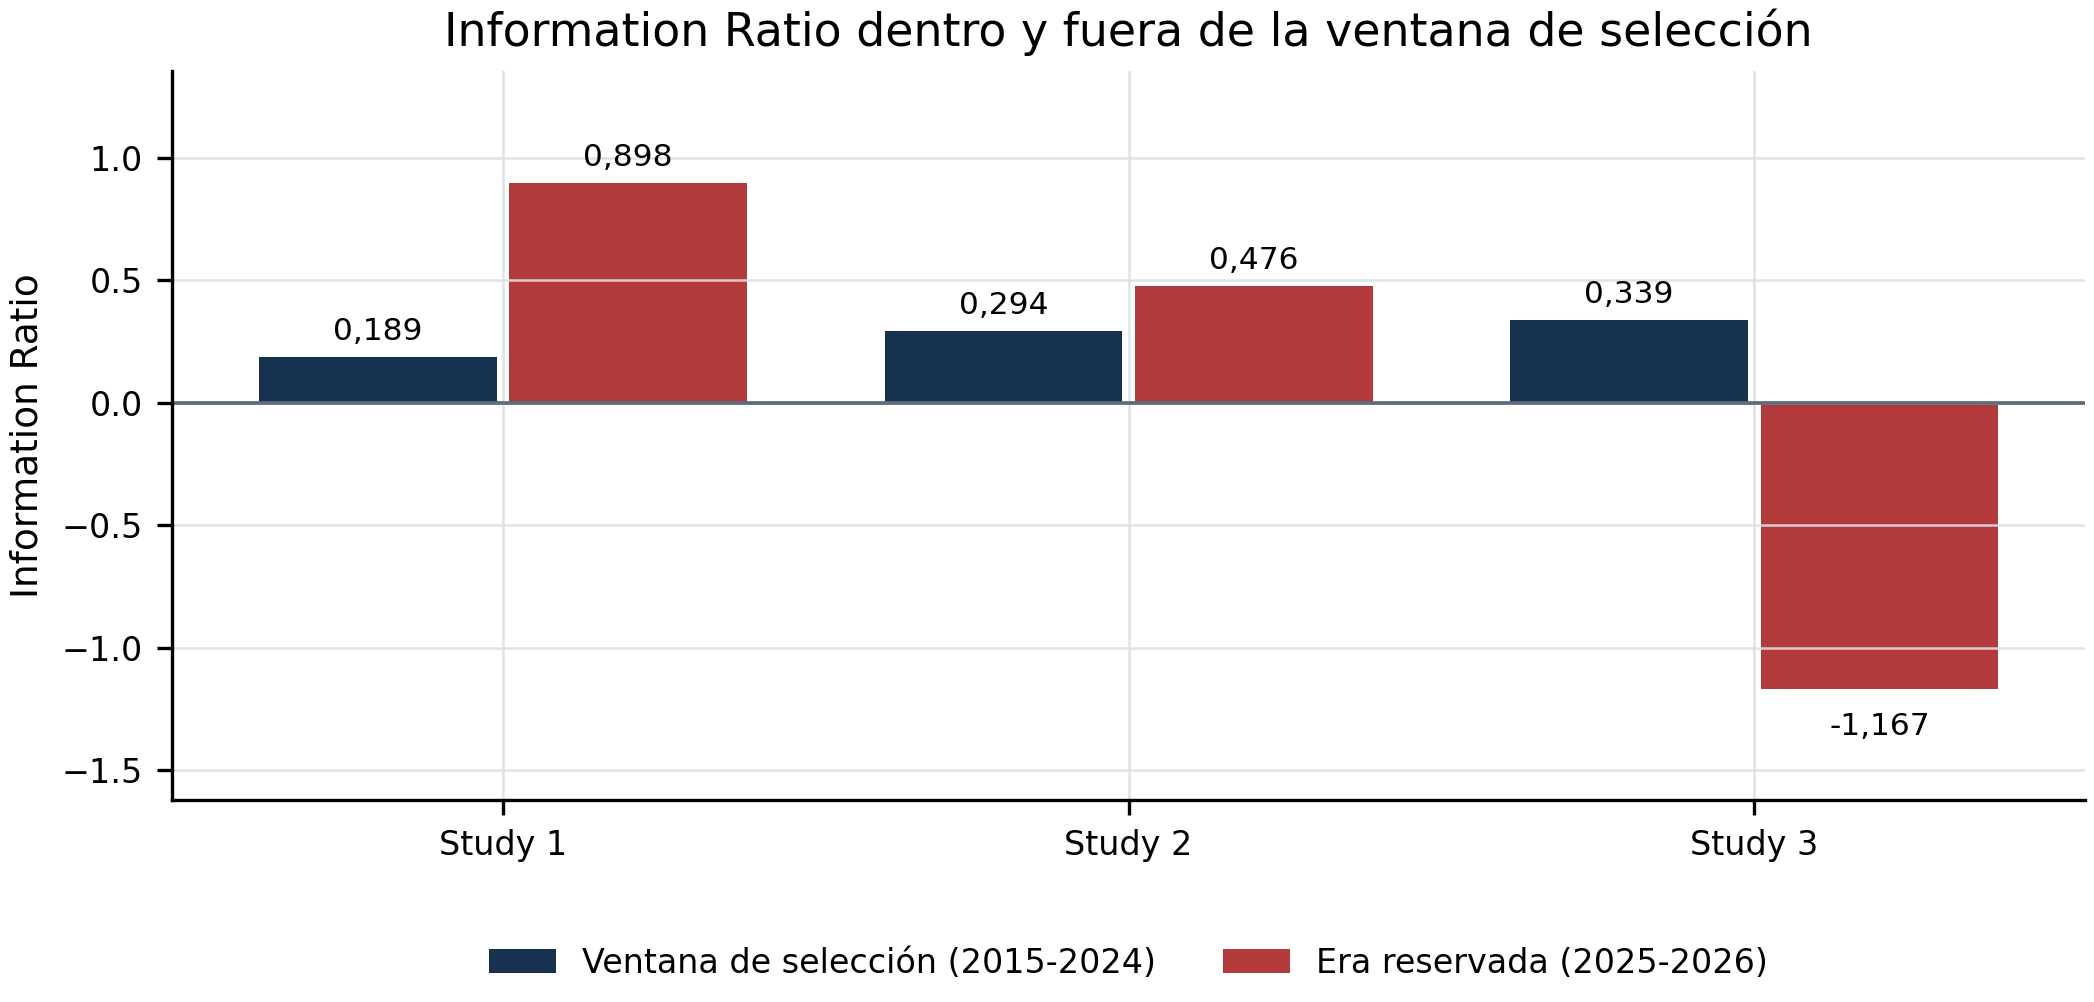
\includegraphics[width=0.92\textwidth]{assets/f09_seleccion_vs_reservada.png}
  \caption{Information Ratio dentro y fuera de la ventana de selección, pasada a pasada de la
  cadena. Fuente: \artefacto{evidence/summary.json} de las tres pasadas.}
  \label{fig:seleccion-vs-reservada}
\end{figure}

La Figura~\ref{fig:seleccion-vs-reservada} documenta el problema que la optimización de cartera
vino a resolver, y conviene leerla antes que la solución. Las tres pasadas de la cadena mejoran
monótonamente dentro de la ventana de selección --- 0,189, 0,294 y 0,339 de Information Ratio --- y
\emph{se degradan} monótonamente fuera de ella: 0,898, 0,476 y $-1{,}167$. Con la cartera por
defecto, la tercera pasada, que es la mejor de la cadena en selección, es la peor con diferencia en
la era reservada, donde pierde un 11,29\,\% frente al índice sin batirlo ni un solo año. Es la firma
clásica del sobreajuste por búsqueda: cada pasada aprendía algo más sobre la ventana con la que se
decidía y algo menos sobre el mundo.

El hallazgo es que esa degradación \textbf{no procedía del modelo}. Con la cartera optimizada, la
misma señal, sin reentrenar nada y sin tocar una sola variable predictiva, obtiene en la era
reservada un exceso de $+2{,}56$\,\% y un Information Ratio de $+0{,}304$, batiendo al índice en la
mitad de los años en lugar de en ninguno. La ordenación transversal siempre había sido válida fuera
de muestra --- su Rank-IC en esa era es $+0{,}0441$, positivo aunque menor que en selección ---; lo
que fallaba era la maquinaria que la convertía en posiciones.

Este resultado exige dos cautelas explícitas y el trabajo no las oculta. La primera es de tamaño
muestral: la era reservada abarca seis cohortes y aproximadamente 1,41 años de cartera, de modo que
«bate en la mitad de los años» significa uno de dos, y ningún contraste construido sobre esa
cantidad de datos puede ser concluyente. La segunda es de multiplicidad: la cartera ganadora es la
mejor de 1.728, y aunque ninguna de ellas pudo ver la era reservada durante la selección, el hecho
de que la ganadora generalice no queda demostrado por un único periodo de confirmación. Lo que sí
puede afirmarse, y es lo que se afirma, es que la hipótesis «la señal no se traslada a rentabilidad
fuera de muestra» queda desmentida en las condiciones medidas, y que la gestión de cartera --- no la
capacidad predictiva --- era el cuello de botella.

\subsection*{Los ocho perfiles con la cartera ganadora}

\begin{table}[H]
  \centering
  \small
  \caption{Los ocho perfiles de inversor evaluados con la cartera ganadora.}
  \label{tab:perfiles-cartera}
  \begin{tabular}{lrrrrrr}
\toprule
Perfil & IR sel. & Exceso sel. & Turnover & Efectivo & IR reserv. & Exceso reserv. \\
\midrule
balanced & 0,844 & 6,97\% & 3,24 & 0,00\% & 0,304 & 2,56\% \\
defensive & 0,570 & 3,73\% & 2,51 & 0,00\% & -0,607 & -5,70\% \\
quality & 0,312 & 2,06\% & 3,40 & 0,00\% & -0,635 & -9,09\% \\
growth & 0,212 & 1,04\% & 3,93 & 0,00\% & 0,318 & 4,14\% \\
value & 0,190 & 1,16\% & 3,82 & 0,00\% & -0,513 & -4,94\% \\
garp & 0,112 & 0,51\% & 3,89 & 0,00\% & -0,779 & -8,76\% \\
contrarian & 0,057 & -0,40\% & 4,33 & 0,00\% & 0,414 & 4,44\% \\
momentum & 0,017 & -0,77\% & 5,98 & 0,00\% & 1,889 & 41,59\% \\
\bottomrule
\end{tabular}

  \caption*{Fuente: \artefacto{portfolio\_profiles.parquet}. Las columnas de selección se miden
  sobre 2015--2024 y las de la era reservada sobre 2025--2026. Ningún perfil se elige por su
  Information Ratio.}
\end{table}

Los perfiles se reevalúan con la cartera ya elegida porque responden a una pregunta distinta: cómo
le habría ido a cada estilo de inversor con la mejor gestión disponible. No compiten en la rejilla,
y la razón es de principio y no de conveniencia: un perfil \emph{reordena la señal} --- sustituye el
\texttt{meta\_rank} y recalibra el alfa esperado ---, de modo que opera en el plano predictivo.
Elegir perfil por su Information Ratio sería seleccionar el estilo de inversor por su rentabilidad
conocida, exactamente la práctica que el protocolo prohíbe.

La lectura relevante de la Tabla~\ref{tab:perfiles-cartera} no es cuál gana, sino que \emph{ninguno
mejora a la señal sin reordenar}. El perfil \texttt{balanced} --- el único que no altera el
resultado del meta-agente --- domina la ventana de selección con un Information Ratio de 0,844
frente al 0,570 del siguiente, y los siete estilos que sí reordenan la señal quedan por debajo, dos
de ellos con exceso negativo. Es un indicio, con las reservas propias de una comparación no
controlada, de que la ordenación aprendida ya contiene lo que los perfiles intentan imponer desde
fuera.

La era reservada, en cambio, invierte el orden casi por completo, y el dato merece reportarse
precisamente porque incomoda: \texttt{momentum}, el peor perfil de la ventana de selección con un
Information Ratio de 0,017, es el mejor con diferencia en 2025--2026, con 1,889 y un exceso del
41,59\,\%. La tentación de leer ahí un hallazgo debe resistirse. Seis cohortes no permiten ordenar
ocho estilos de inversión, y un periodo tan corto está dominado por qué régimen de mercado le tocó
en suerte a cada sesgo. Lo que la comparación sí sugiere, y de forma consistente con el resto del
capítulo, es que el orden entre perfiles no es una propiedad estable de la señal sino del régimen, y
que por eso mismo el protocolo hace bien en no elegir perfil por su rentabilidad.

\subsection*{De dónde procede la rotación}

Un turnover del 359\,\% anualizado exige explicación. La Tabla~\ref{tab:ordenes} lo descompone por
motivo declarado de cada orden, y la Figura~\ref{fig:ordenes} lo representa.

\begin{table}[H]
  \centering
  \small
  \caption{Descomposición del flujo de cartera por motivo de orden.}
  \label{tab:ordenes}
  \begin{tabular}{lrrr}
\toprule
Motivo de la orden & Órdenes & \% del flujo & Coste \\
\midrule
net\_edge\_over\_worst & 40 & 36,5\% & 3,43 \\
displaced\_by\_net\_edge & 40 & 35,0\% & 3,31 \\
rebalance & 61 & 17,6\% & 2,18 \\
initial\_fill & 8 & 7,3\% & 0,30 \\
cash\_floor\_fill & 2 & 1,8\% & 0,25 \\
missing\_current\_score & 2 & 1,8\% & 0,24 \\
\textbf{Total} & \textbf{153} & \textbf{100,0\%} & \textbf{9,70} \\
\bottomrule
\end{tabular}

  \caption*{Fuente: \artefacto{evidence/orders.parquet}. El flujo es la suma de $|\Delta w|$ de cada
  orden. El coste agrega comisión y \textit{slippage} efectivamente cargados.}
\end{table}

\begin{figure}[H]
  \centering
  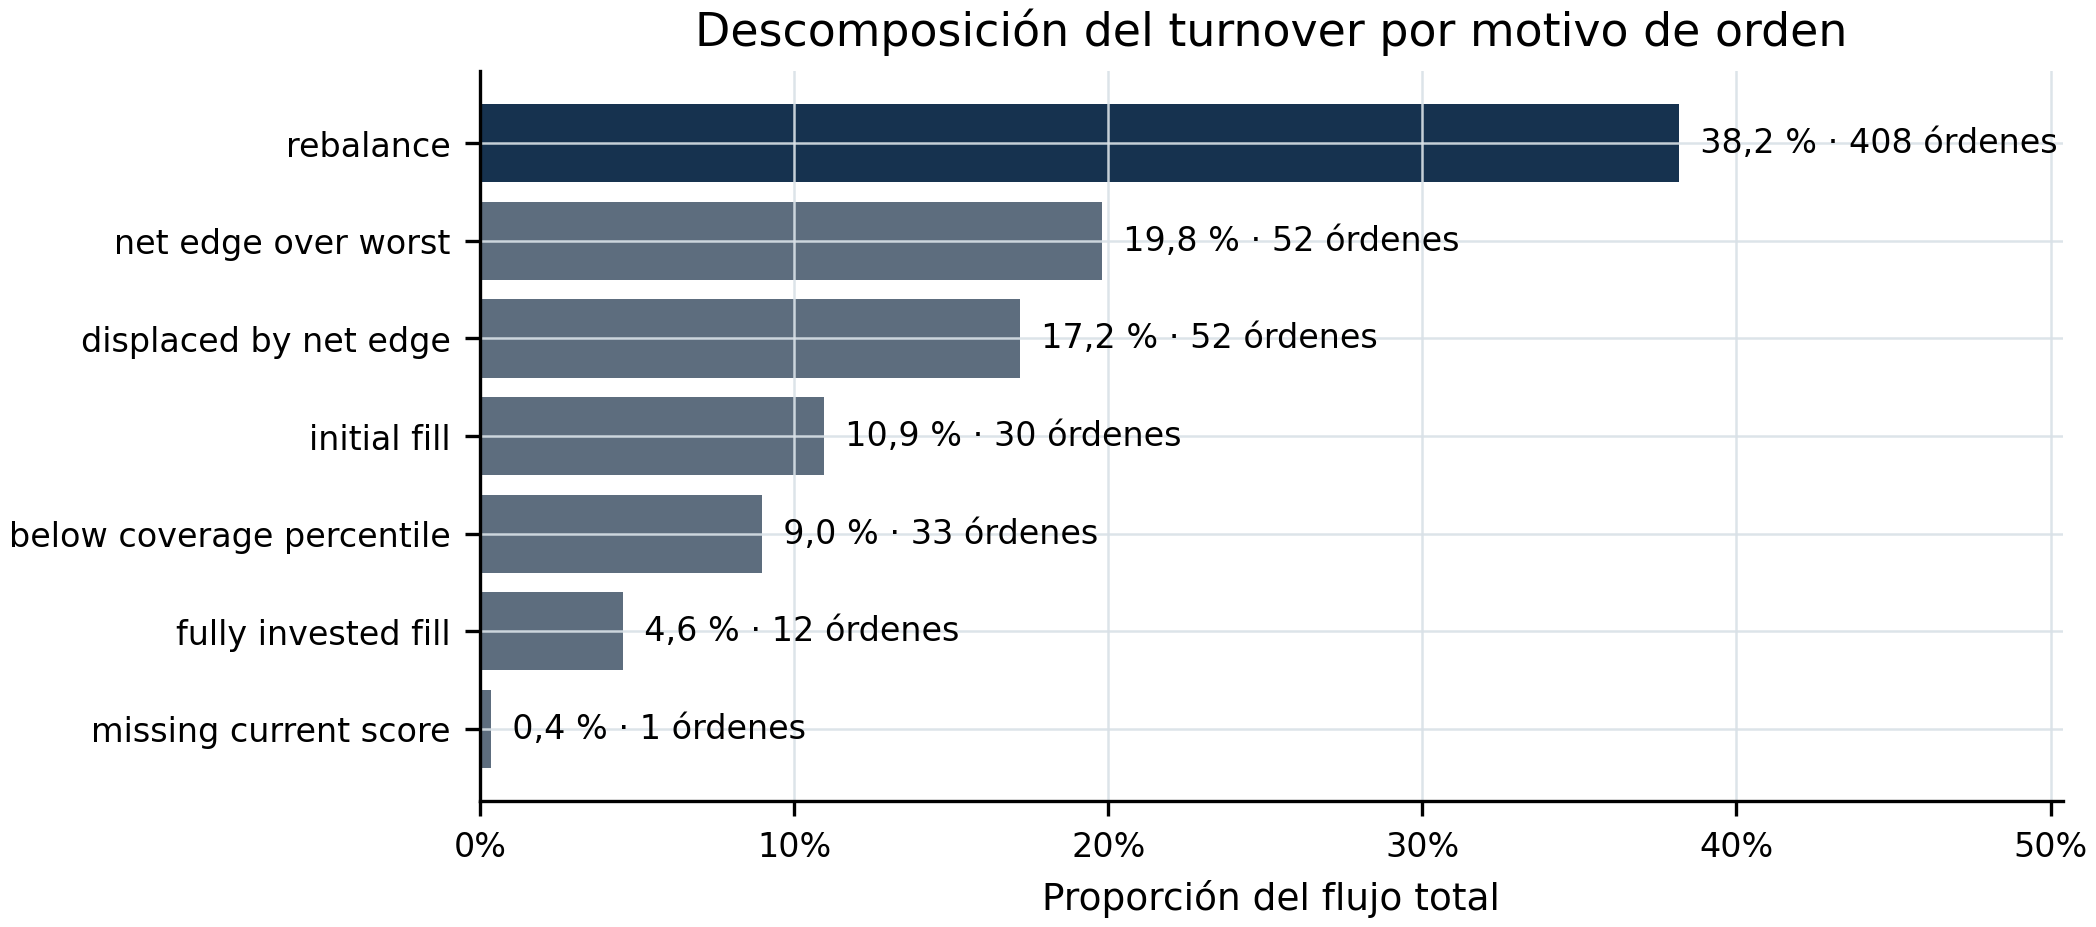
\includegraphics[width=0.92\textwidth]{assets/f07_ordenes.png}
  \caption{Origen del turnover por motivo de orden. Fuente: \artefacto{evidence/orders.parquet}.}
  \label{fig:ordenes}
\end{figure}

Los dos motivos de rotación --- \texttt{net\_edge\_over\_worst} y \texttt{displaced\_by\_net\_edge},
que son las dos caras de una misma operación --- suman el 56,5\,\% del flujo. El
\texttt{rebalance} aporta un 20,2\,\%, las compras iniciales un 13,5\,\% y las salidas por alfa
insuficiente un 10,0\,\%. La causa raíz no es un umbral mal calibrado sino algo estructural: el
sistema \emph{re-decide todos los meses} sobre una señal cuyo horizonte es de \emph{doce}. Cada
snapshot vuelve a comparar las posiciones en cartera con todo el universo, y basta una diferencia neta
que supere el umbral de rotación para que se ejecute un intercambio que la señal, a doce meses
vista, quizá no habría pedido.

De ahí que la palanca estructural sea \artefacto{snapshot\_step\_months}, que reduciría la rotación
en un factor cercano a tres. Pero es una variable \emph{predictiva}: cambiarla obligaría a rehacer
la selección secuencial completa, y de hecho fue la primera decisión del estudio, donde la cadencia
mensual ganó con una ventaja pareada de $+0{,}0208$ frente a la trimestral. El sistema se encuentra
así ante un conflicto real entre dos objetivos legítimos --- más cohortes para decidir mejor frente
a menos rotación para implementar mejor --- que este trabajo documenta pero no resuelve.

\subsection*{Rotación, coste y exceso año a año}

La Figura~\ref{fig:transferencia} cruza las tres magnitudes por año.

\begin{figure}[H]
  \centering
  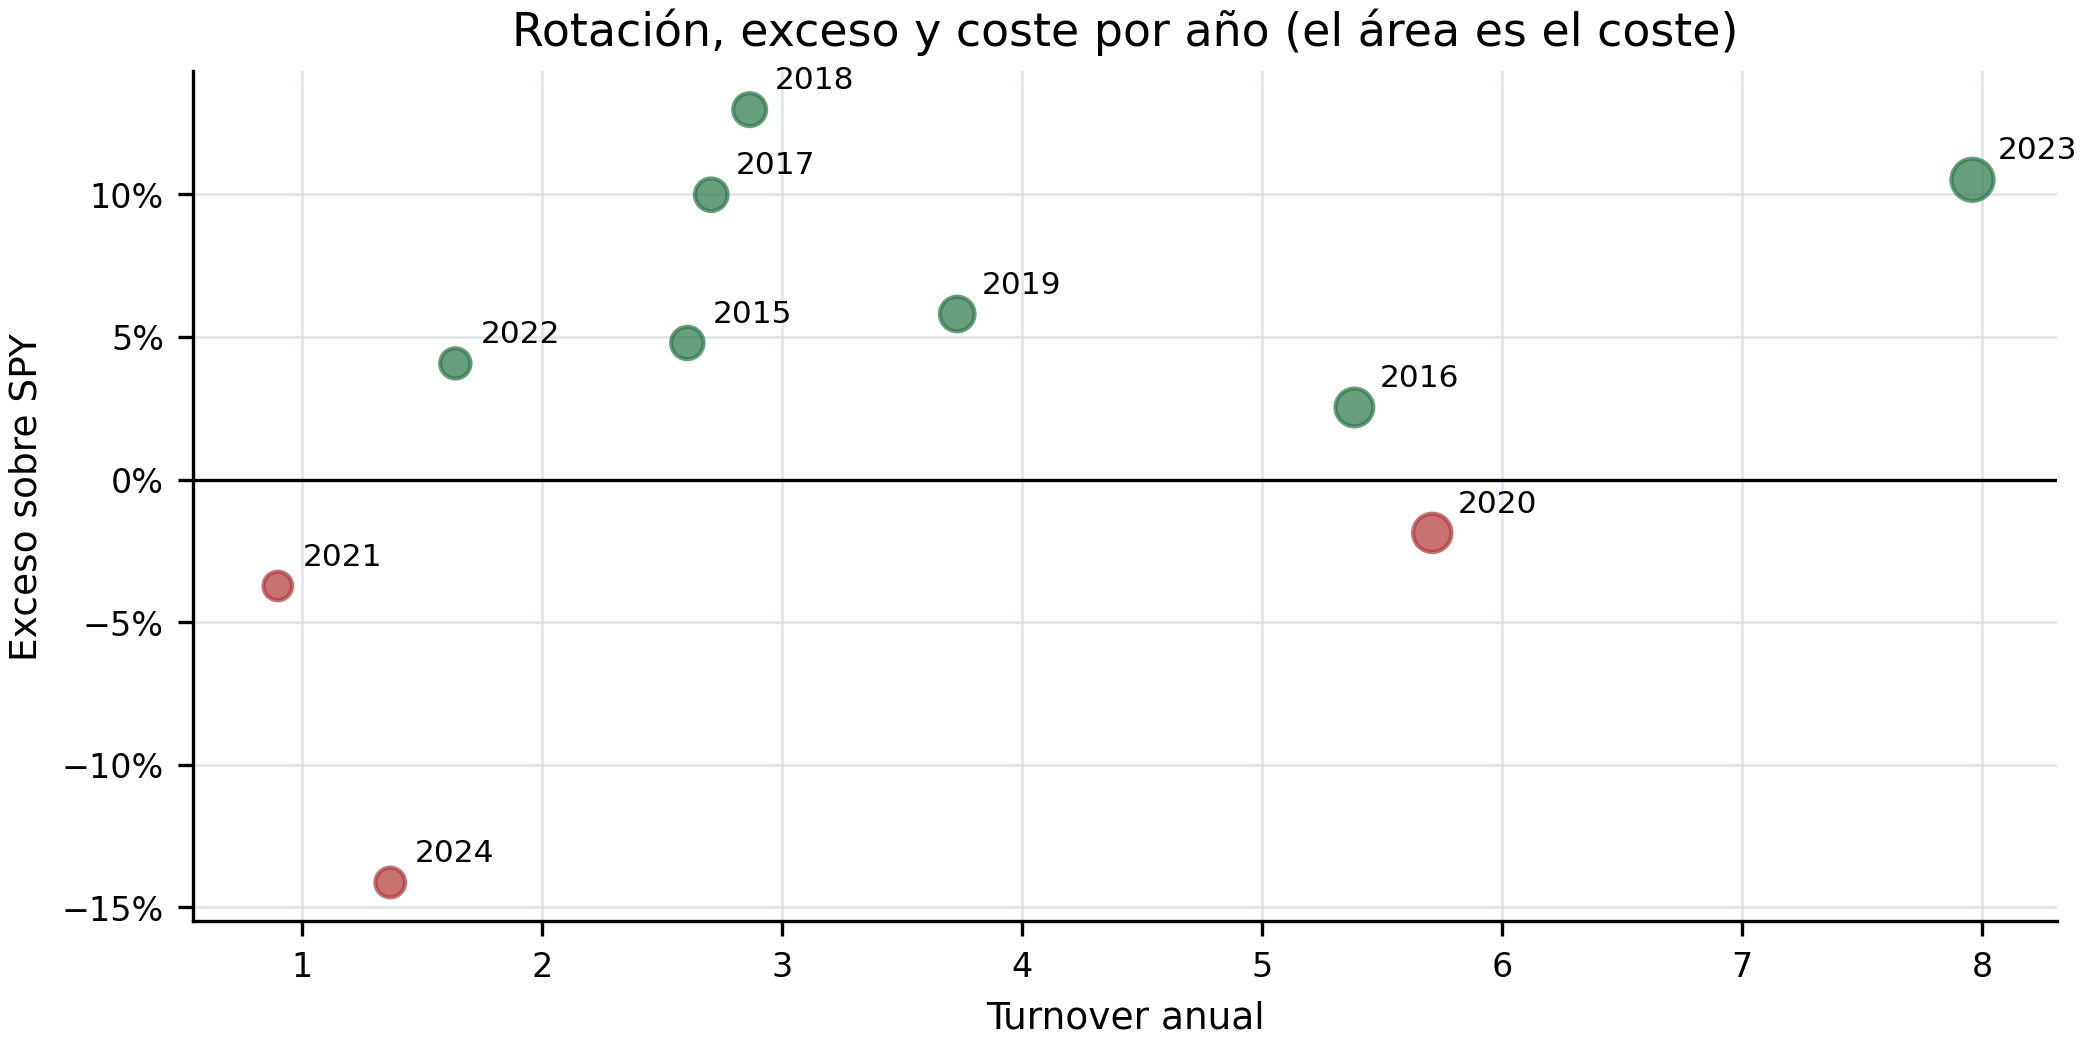
\includegraphics[width=0.94\textwidth]{assets/f07_transferencia.png}
  \caption{Rotación, exceso sobre SPY y coste por año, para la cartera del Model Study. El área de
  cada punto es proporcional al coste soportado. Fuente: \artefacto{attribution.json}, campo
  \texttt{transfer.by\_year}; el Portfolio Study no recalcula la transferencia.}
  \label{fig:transferencia}
\end{figure}

Una precisión sobre las fuentes, para que la comparación entre esta figura y la
Tabla~\ref{tab:anual} no induzca a error: son dos series próximas pero no idénticas. La tabla anual
usa \artefacto{evidence/annual\_metrics.parquet}, cuya alfa se calcula sobre el año natural
completo; la figura usa el campo de transferencia de \artefacto{attribution.json}, que agrega por
cohortes. Para 2024 la primera da $-11{,}63$\,\% y la segunda $-12{,}33$\,\%. La diferencia es de
agregación, no de resultado, pero conviene no citar ambas como si fueran la misma cifra.

No hay una relación monótona entre rotar más y obtener más exceso, lo que descarta que el turnover
esté comprando rentabilidad. 2017 y 2023, los dos mejores años en alfa (25,35\,\% y 18,57\,\%),
tienen rotaciones distintas (3,08 y 4,69), y 2024 rotó todavía más (4,76) para un alfa de apenas
2,07\,\%. En el otro extremo, el peor año de la ventana, 2022, tuvo la rotación más baja de toda la
serie (1,20): su pérdida frente al índice no se explica por costes sino por composición. El coste
acumulado de 4,74 puntos porcentuales sobre la ventana no es despreciable frente a un exceso
geométrico de 6,97\,\%: en términos brutos, antes de costes, la ventaja sería sustancialmente mayor,
y es la implementación la que se lleva una parte apreciable.

Conviene notar que la optimización de cartera redujo la rotación al mismo tiempo que elevó el
exceso --- de 3,58 a 3,24 veces al año ---, de modo que la mejora no se compró rotando más. Es
coherente con lo que muestra la Figura~\ref{fig:cartera-rejilla}: en la nube de las 1.728 carteras,
el Information Ratio y el turnover no guardan una relación clara, y las mejores combinaciones
aparecen repartidas por todo el rango de rotación.

\section{Implicación para el diseño de cartera}

El mejor perfil es \texttt{balanced}, precisamente el que no reordena el resultado del meta. Esta
comparación tiene valor causal limitado pero controlado: todos los perfiles parten de la misma señal,
por lo que sus diferencias se atribuyen a la regla de construcción y no al reentrenamiento de otro
modelo. Los perfiles con sesgos agresivos elevan a menudo el turnover y reducen el exceso. El caso
de \texttt{momentum}, peor perfil y agente más débil, advierte contra imponer una narrativa de estilo
sobre un ranking que ya incorporó esa información.

El coeficiente de transferencia de 0,328 concentraba la agenda práctica, y este trabajo la ha
recorrido hasta el final. La señal no era el único cuello de botella: una cartera long-only no puede
explotar la cola inferior, paga costes por rotar y debe limitar concentración. La rejilla de la
Sección~\ref{sec:cartera-rejilla} evaluó exactamente eso --- tamaño de cartera, reparto de pesos,
efectivo, tenencia mínima, suelo de cobertura y tolerancia de deriva --- sin reabrir la selección
predictiva, y encontró una configuración que multiplica por 2,5 el Information Ratio de la ventana
de selección y, sobre todo, cambia el signo del resultado en la era reservada.

La implicación de diseño es más fuerte de lo que este capítulo podía afirmar antes de existir el
Portfolio Study: en este sistema, la construcción de cartera no era un detalle de implementación
sino la variable que decidía si la señal servía para algo. Dos carteras alimentadas por el mismo
modelo, con la misma señal y sobre el mismo panel, produjeron en la era reservada un exceso de
$-11,29$\% y otro de $+2,56$\%. Ninguna conclusión sobre la utilidad práctica de un sistema
predictivo es interpretable sin declarar con qué cartera se midió.
